%% 
%% Copyright 2007-2024 Elsevier Ltd
%% 
%% This file is part of the 'Elsarticle Bundle'.
%% ---------------------------------------------
%% 
%% It may be distributed under the conditions of the LaTeX Project Public
%% License, either version 1.3 of this license or (at your option) any
%% later version.  The latest version of this license is in
%%    http://www.latex-project.org/lppl.txt
%% and version 1.3 or later is part of all distributions of LaTeX
%% version 1999/12/01 or later.
%% 
%% The list of all files belonging to the 'Elsarticle Bundle' is
%% given in the file `manifest.txt'.
%% 
%% Template article for Elsevier's document class `elsarticle'
%% with numbered style bibliographic references
%% SP 2008/03/01
%% $Id: elsarticle-template-num.tex 249 2024-04-06 10:51:24Z rishi $
%%
\documentclass[final,3p,times,12pt]{elsarticle}
% \usepackage[margin=0.85in]{geometry}
%% Use the option review to obtain double line spacing
%% \documentclass[authoryear,preprint,review,12pt]{elsarticle}
%% Use the options 1p,twocolumn; 3p; 3p,twocolumn; 5p; or 5p,twocolumn
%% for a journal layout:
%% \documentclass[final,1p,times]{elsarticle}
%% \documentclass[final,1p,times,twocolumn]{elsarticle}
%% \documentclass[final,3p,times]{elsarticle}
%% \documentclass[final,3p,times,twocolumn]{elsarticle}
%% \documentclass[final,5p,times]{elsarticle}
%% \documentclass[final,5p,times,twocolumn]{elsarticle}
%% For including figures, graphicx.sty has been loaded in
%% elsarticle.cls. If you prefer to use the old commands
%% please give \usepackage{epsfig}
%% The amssymb package provides various useful mathematical symbols
\usepackage{amssymb,xcolor}
%% The amsmath package provides various useful equation environments.
\usepackage{amsmath,booktabs}
%% The amsthm package provides extended theorem environments
%% \usepackage{amsthm}

%% The lineno packages adds line numbers. Start line numbering with
%% \begin{linenumbers}, end it with \end{linenumbers}. Or switch it on
%% for the whole article with \linenumbers.
%% \usepackage{lineno}

\journal{Renewable and Sustainable Energy Reviews}

\begin{document}

\begin{frontmatter}

%% Title, authors and addresses

%% use the tnoteref command within \title for footnotes;
%% use the tnotetext command for theassociated footnote;
%% use the fnref command within \author or \affiliation for footnotes;
%% use the fntext command for theassociated footnote;
%% use the corref command within \author for corresponding author footnotes;
%% use the cortext command for theassociated footnote;
%% use the ead command for the email address,
%% and the form \ead[url] for the home page:
%% \title{Title\tnoteref{label1}}
%% \tnotetext[label1]{}
%% \author{Name\corref{cor1}\fnref{label2}}
%% \ead{email address}
%% \ead[url]{home page}
%% \fntext[label2]{}
%% \cortext[cor1]{}
%% \affiliation{organization={},
%%             addressline={},
%%             city={},
%%             postcode={},
%%             state={},
%%             country={}}
%% \fntext[label3]{}

\title{A Data-Driven Qualitative Review of Thermal Comfort Studies: Bridging the Gap Between Western and Eastern Perspectives}

%% use optional labels to link authors explicitly to addresses:
%% \author[label1,label2]{}
%% \affiliation[label1]{organization={},
%%             addressline={},
%%             city={},
%%             postcode={},
%%             state={},
%%             country={}}
%%
%% \affiliation[label2]{organization={},
%%             addressline={},
%%             city={},
%%             postcode={},
%%             state={},
%%             country={}}

\author[inst1]{Yu Chang}

\affiliation[inst1]{organization={Department of Architecture, Faculty of Architecture, the University of Hong Kong},%Department and Organization
            addressline={Knowles Building}, 
            city={Hong Kong SAR},
            % postcode={00000}, 
            % state={State One},
            country={China}}
\affiliation[inst2]{organization={Department of Theoretical and Applied Sciences, eCampus University},,%Department and Organization
            %addressline={Knowles Building}, 
            city={Novedrate (CO)},
            % postcode={00000}, 
            % state={State One},
            country={Italy}}

\author[inst1]{Hongshan Guo}
\author[inst1]{Yichun Li}
\author[inst2]{Ilaria Pigliautile}
\author[inst1]{Binlin Chi}

%% Abstract
\begin{abstract}

In the face of increasing availability of global thermal comfort datasets, there remains a critical gap in how personal, contextual, and environmental variables are comparatively analyzed across cultural and regional contexts. This study conducts a data-driven qualitative review of 88 thermal comfort studies drawn from the ASHRAE Global Thermal Comfort Database and the Chinese Thermal Comfort Dataset, focusing on the depth and consistency of parameter usage in existing literature. Studies were systematically evaluated along 15 variables grouped into personal characteristics, contextual parameters, and PMV model inputs, assigning scores on a scale from 0 to 3 to reflect their level of consideration.

Our findings reveal that personal parameters such as height and weight are the least reported (75.6\% of studies omitted them), while contextual parameters like season and operation mode received greater attention. Notably, only 34.9\% of studies fully account for metabolic rate variation in PMV modeling, while MRT is assumed rather than measured in over 55\% of reviewed cases. Using the Chinese dataset, we also derive region-specific adaptive comfort models, with regression slopes ranging from 0.196 (severe cold zone) to 0.819 (hot summer/warm winter zone), underscoring significant geographic variation in thermal adaptation. These findings not only support improved comfort modeling but also inform more energy-efficient, renewables-aligned HVAC control strategies.

This review highlights the lack of standardized classification systems as a key barrier to integrated analysis. We advocate for harmonized parameter definitions and expanded demographic coverage to enhance the accuracy and cultural relevance of future comfort models.

\end{abstract}

%% Keywords
\begin{keyword}
indoor thermal environment \sep thermal comfort database \sep personal characteristics \sep contextual parameters \sep inputs for PMV calculation
%% keywords here, in the form: keyword \sep keyword
%% PACS codes here, in the form: \PACS code \sep code
%% MSC codes here, in the form: \MSC code \sep code
%% or \MSC[2008] code \sep code (2000 is the default)

\end{keyword}

\end{frontmatter}

%% Add \usepackage{lineno} before \begin{document} and uncomment 
%% following line to enable line numbers
%% \linenumbers

%% main text
%%

%% Use \section commands to start a section
\section{Introduction}
\label{sec1}

In an era where precision engineering promises optimal indoor environments, many building 
occupants still grapple with discomfort, revealing a disconnection between technological solutions and human thermal experiences. This study seeks to bridge this gap by analyzing global thermal comfort datasets. On one hand, we have the promise by the multitude of options that claims to achieve perfect temperature control, humidity management, explicit air quality control, and energy conservation \cite{almindeelEnergyThermalComfort2024,halhoulmerabetIntelligentBuildingControl2021,yangThermalComfortBuilding2014}. On the other hand, we face the reality of human experience: occupants feeling overheated or overcooled in spaces that are supposedly ‘optimized’ for their comfort, further highlighting waste of energy and available resources, in general \cite{djamilaIndoorThermalComfort2017,taleghaniReviewThermalComfort2013,zhouOpportunitiesChallengesUsing2023}. This contrast between the two worlds raises a critical question: what is the true relationship between technological capabilities and human needs? How to better shape the first one to meet the latter can be investigated via data mining, taking advantage of big data availabilities?

Recognizing this disparity between theoretical expectations and real-world experiences, we sought to investigate how we could best leverage the only two publicly available Thermal Comfort Databases (TCDBs)—the ASHRAE Global Thermal Comfort Database \cite{foldvarylicinaDevelopmentASHRAEGlobal2018a} and the Chinese Thermal Comfort Dataset \cite{yangChineseThermalComfort2023}. These repositories provide invaluable insights into how different people experience thermal environments. They inform building design principles that not only aim to save energy but also enhance occupant comfort. This broadened the scope of available data, emphasizing the varied thermal preferences and responses observed across different populations \cite{yangResidentialThermalEnvironment2013}. This growing body of research highlights the critical need for developing tools that can adapt building environments to accommodate both individual preferences and localized cultural norms \cite{fengDatadrivenPersonalThermal2022,haghiradAdvancingPersonalThermal2024,wangRevisitingIndividualGroup2020a,karjalainenThermalComfortGender2012,wuMethodEvaluateBuilding2020}. While numerous studies have utilized these databases \cite{al-sharifPredictingThermalPreferences2024,duComparisonThermalComfort2022,liModifiedPredictedMean2025,yangComparativeAnalysisIndoor2024}, there has been limited investigation into how they might reveal cross-sectional traits across regions, climate zones, and demographic groups. Additionally, the extent to which the Predicted Mean Vote (PMV) calculation accounts for various contextual parameters remains underexplored.

Comparing thermal comfort studies across different regions reveals fascinating cultural and contextual nuances \cite{ghaniAssessmentThermalComfort2021,tungOutdoorThermalComfort2014}. For example, how do people in the chilly climates of Northern Europe feel about their indoor winter environments compared to those in the humid cities of Asia? Such studies show that what works in one region might not be suitable in another, revealing gaps in our models that could be filled by incorporating a broader spectrum of human experiences \cite{cheungAnalysisAccuracyPMV2019,lambertiDevelopmentComparisonAdaptive2023,schweikerInfluencePersonalityTraits2016}. This comparative approach is crucial for developing more accurate and universally applicable thermal comfort models that respect the diversity of human preferences.

We aim to address these knowledge gaps by analyzing the two datasets together for commonality and differences. In examining them side-by-side, we are hoping to pinpoint specific areas of misalignments. We investigate which remain unused and to what extent individual occupant differences, though recorded, are underutilized in existing datasets. By integrating diverse thermal comfort datasets from regions with varying climatic and cultural conditions \cite{aljawabraInfluenceHotArid2010,aljawabraThermalComfortUrban2018}, our approach aims to bridge theoretical models with real-world applications, thereby maximizing energy efficiency while respecting individual comfort needs. Tailored thermal comfort models enable more precise control over HVAC systems, leading to significant energy savings. This will allow us to provide insights on how researchers and engineers can best leverage these datasets effectively in the near future.

While thermal comfort research has traditionally focused on occupant well-being \cite{singhProgressThermalComfort2019}, its implications for energy policy are increasingly relevant. Adaptive and personalized comfort models can significantly reduce reliance on rigid HVAC operation, thereby lowering energy demand during peak hours and supporting grid-responsive building operations. This connection is particularly crucial in the context of renewable energy integration, where flexible comfort thresholds can complement variable energy supply. Therefore, improving the contextual accuracy and cultural inclusiveness of comfort models is not only a scientific imperative, but also an energy policy enabler. We hope to contribute to a more sustainable, comfortable, and energy-efficient future, recognizing that thermal comfort is deeply personal and profoundly influenced by cultural and regional contexts. Ultimately, this work seeks to refine thermal comfort models to be more inclusive, ensuring that they serve the global population more effectively and empathetically.  

\section{Literature Review Methodology}
\label{sec1}

\subsection{General Introduction of Two Databases}
\label{subsec1}

The ASHRAE Global Thermal Comfort Database contains a total of 107,463 records, divided into two key datasets. The first dataset, known as the ASHRAE Global Thermal Comfort Database I, was established by De Dear in 1998 \cite{dedearGlobalDatabaseThermal}. It includes 25,617 records collected from 52 field studies conducted between 1988 and 1997, encompassing 884 samples from 160 buildings worldwide. These studies primarily focused on thermal comfort and the role of HVAC systems, laying the groundwork for the development of the adaptive thermal comfort model \cite{dedearDevelopingAdaptiveModel1998}.

The second dataset, ASHRAE Global Thermal Comfort Database II \cite{foldvarylicinaDevelopmentASHRAEGlobal2018a}, comprises 81,846 records and was developed by the Center for the Built Environment at the University of California, Berkeley, in collaboration with the Indoor Environment Quality Laboratory at the University of Sydney. This dataset draws from field studies conducted between 1995 and 2016 across 23 countries and five continents. It represents a wide range of conditions, including four seasons, 16 climate zones, diverse ventilation strategies, and various building types. The dataset includes both objective environmental measurements (e.g., indoor climate data) and subjective responses collected through questionnaires.

Together, these two datasets form a comprehensive resource for studying thermal comfort across diverse climates, seasons, and cultural contexts. They also provide a robust foundation for advancing thermal comfort research and informing the development of ASHRAE standards.

Although the ASHRAE database includes data from the Chinese region, the sample size is limited, accounting for only 7.7\% of the total records. China spans multiple climatic zones, each with varying thermal comfort requirements, necessitating adjustments in cooling/heating strategies. To fill this gap, the Chinese Thermal Comfort Dataset \cite{yangChineseThermalComfort2023} was established in 2018, comprising 41,977 entries covering five typical climatic zones in China, four building types, and three HVAC operation modes. The database is categorized into three levels corresponding to indoor thermal environment parameters obtained directly from original research data, subjective evaluations at all levels, and indoor thermal environment derived parameters obtained through calculation. This database can further be used to develop adaptive models tailored to China, explore thermal comfort differences among residents in different climatic regions, and provide guidance for efficient energy utilization. The data availability heatmap for the two databases is shown in Figure~\ref{1} with key columns, whereas the full data availability heatmap can be found in Appendix with Figure~\ref{fig:fullavail}. Figure~\ref{1} presents a condensed view of selected columns from the complete ASHRAE and Chinese datasets to highlight availability trends. Neither Figure~\ref{1} nor Figure~\ref{fig:fullavail} reflect any sampling or truncation at the row level. Figure~\ref{fig:czrecords} shows the number of records within each climate zone in the ASHRAE and Chinese thermal comfort databases, respectively.

\begin{figure}[h!]
    \centering
    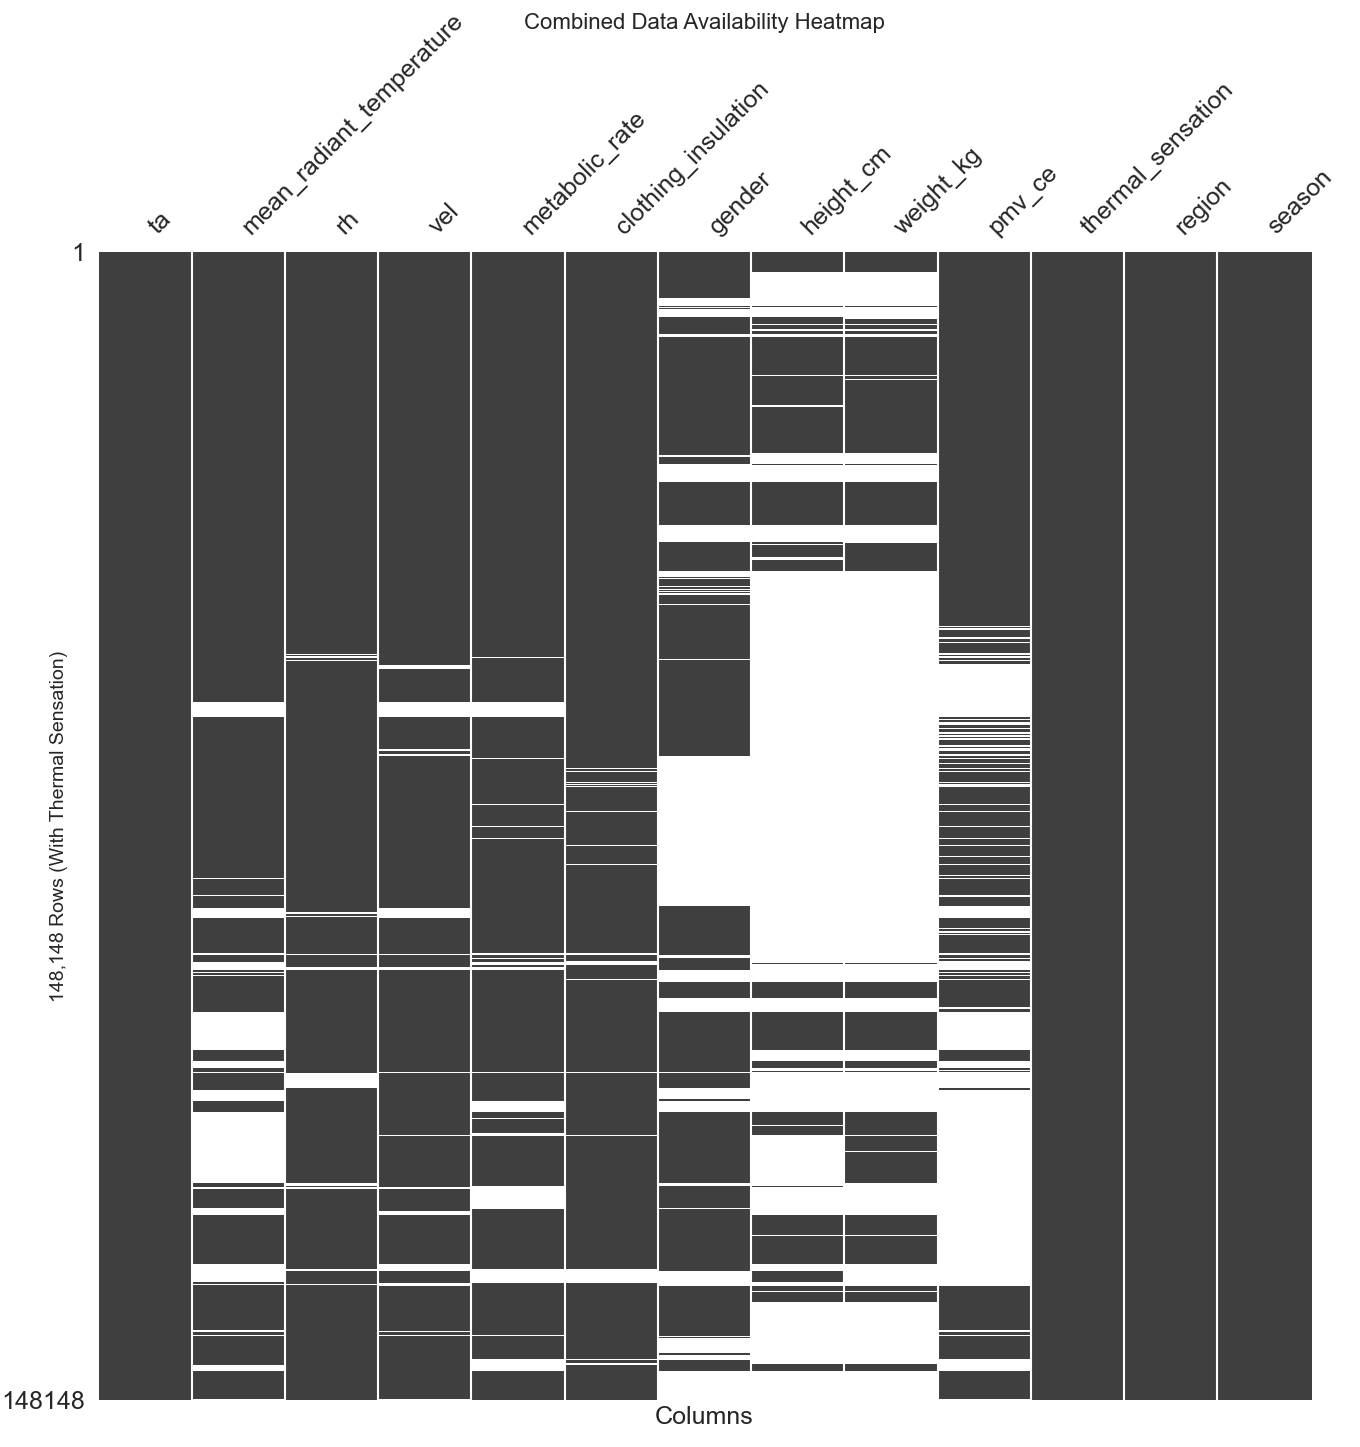
\includegraphics[width=0.85\linewidth]{overall heatmap.png}
    \caption{Data availability heatmap for ASHRAE and Chinese thermal comfort database (selected columns)}
    \label{1}
\end{figure}

\subsection{Selection and Scope of Studies}
\label{subsec1}

In this review paper, the methodology involved a systematic approach to data collection, literature screening, and comparative analysis. The initial step involved collecting articles from both the ASHRAE and Chinese thermal comfort databases. Specifically, 52 articles were gathered from the ASHRAE database, and 28 articles were sourced from the Chinese database. Articles that were outdated or inaccessible were excluded from the review. Following this, any duplicate articles identified between the two databases were removed, resulting in a refined dataset. An additional set of 8 articles that utilized both databases was identified through Google Scholar using keywords such as “thermal comfort database”, “PMV”, “PPD”, “Machine learning”, “adaptive model”, and other related terms. The process of the selection of studies is shown in Figure~\ref{2}.

With reference to the standardized spreadsheet format in Chinese thermal comfort database \cite{yangChineseThermalComfort2023}, the research team created an updated one to record reviewed articles in three sets. The basic bibliometric structure contains four main categories: basic information (Section A), personal characteristics (Section B), contextual parameters (Section C), and inputs for PMV calculation (Section D), as shown in Table~\ref{table 1}. In comparison with the Chinese format, our emphasis lies on the original countries or regions from which the literature data is acquired for Section A. To better understand the geographical influence on thermal comfort, we expanded Section A to include country and region, which was made possible by the mapping provided by both databases. Moving onward to section B, building upon the original four personal characteristics of height, weight, age, and gender, we introduced a new dimension - BMI (Body Mass Index), concentrating on individual differences in the PMV model. In section C, we focused on four contextual parameters, climate zone, season from the basic identifiers (Part A), and building type plus operation model from the Building Information (Part B) as designated in the Chinese database: for records in the ASHRAE database, we mapped these columns out using the accompanying metadata that was published alongside the experiment records. Our objective is to determine whether these four contextual parameters are fully analyzed and explored according to various categories from the thermal comfort database records. The final section, Section D, comprises six fundamental inputs for PMV calculation. The purpose is to confirm the accuracy of the PMV values at the source, specifically assessing whether these input parameters are treated as variables rather than constants.

By following this structured approach, this review aimed to provide a comprehensive understanding of the thermal comfort research as represented in the AHRAE and Chinese databases, as well as studies utilizing these databases.

\begin{figure}[h!]
    \centering
    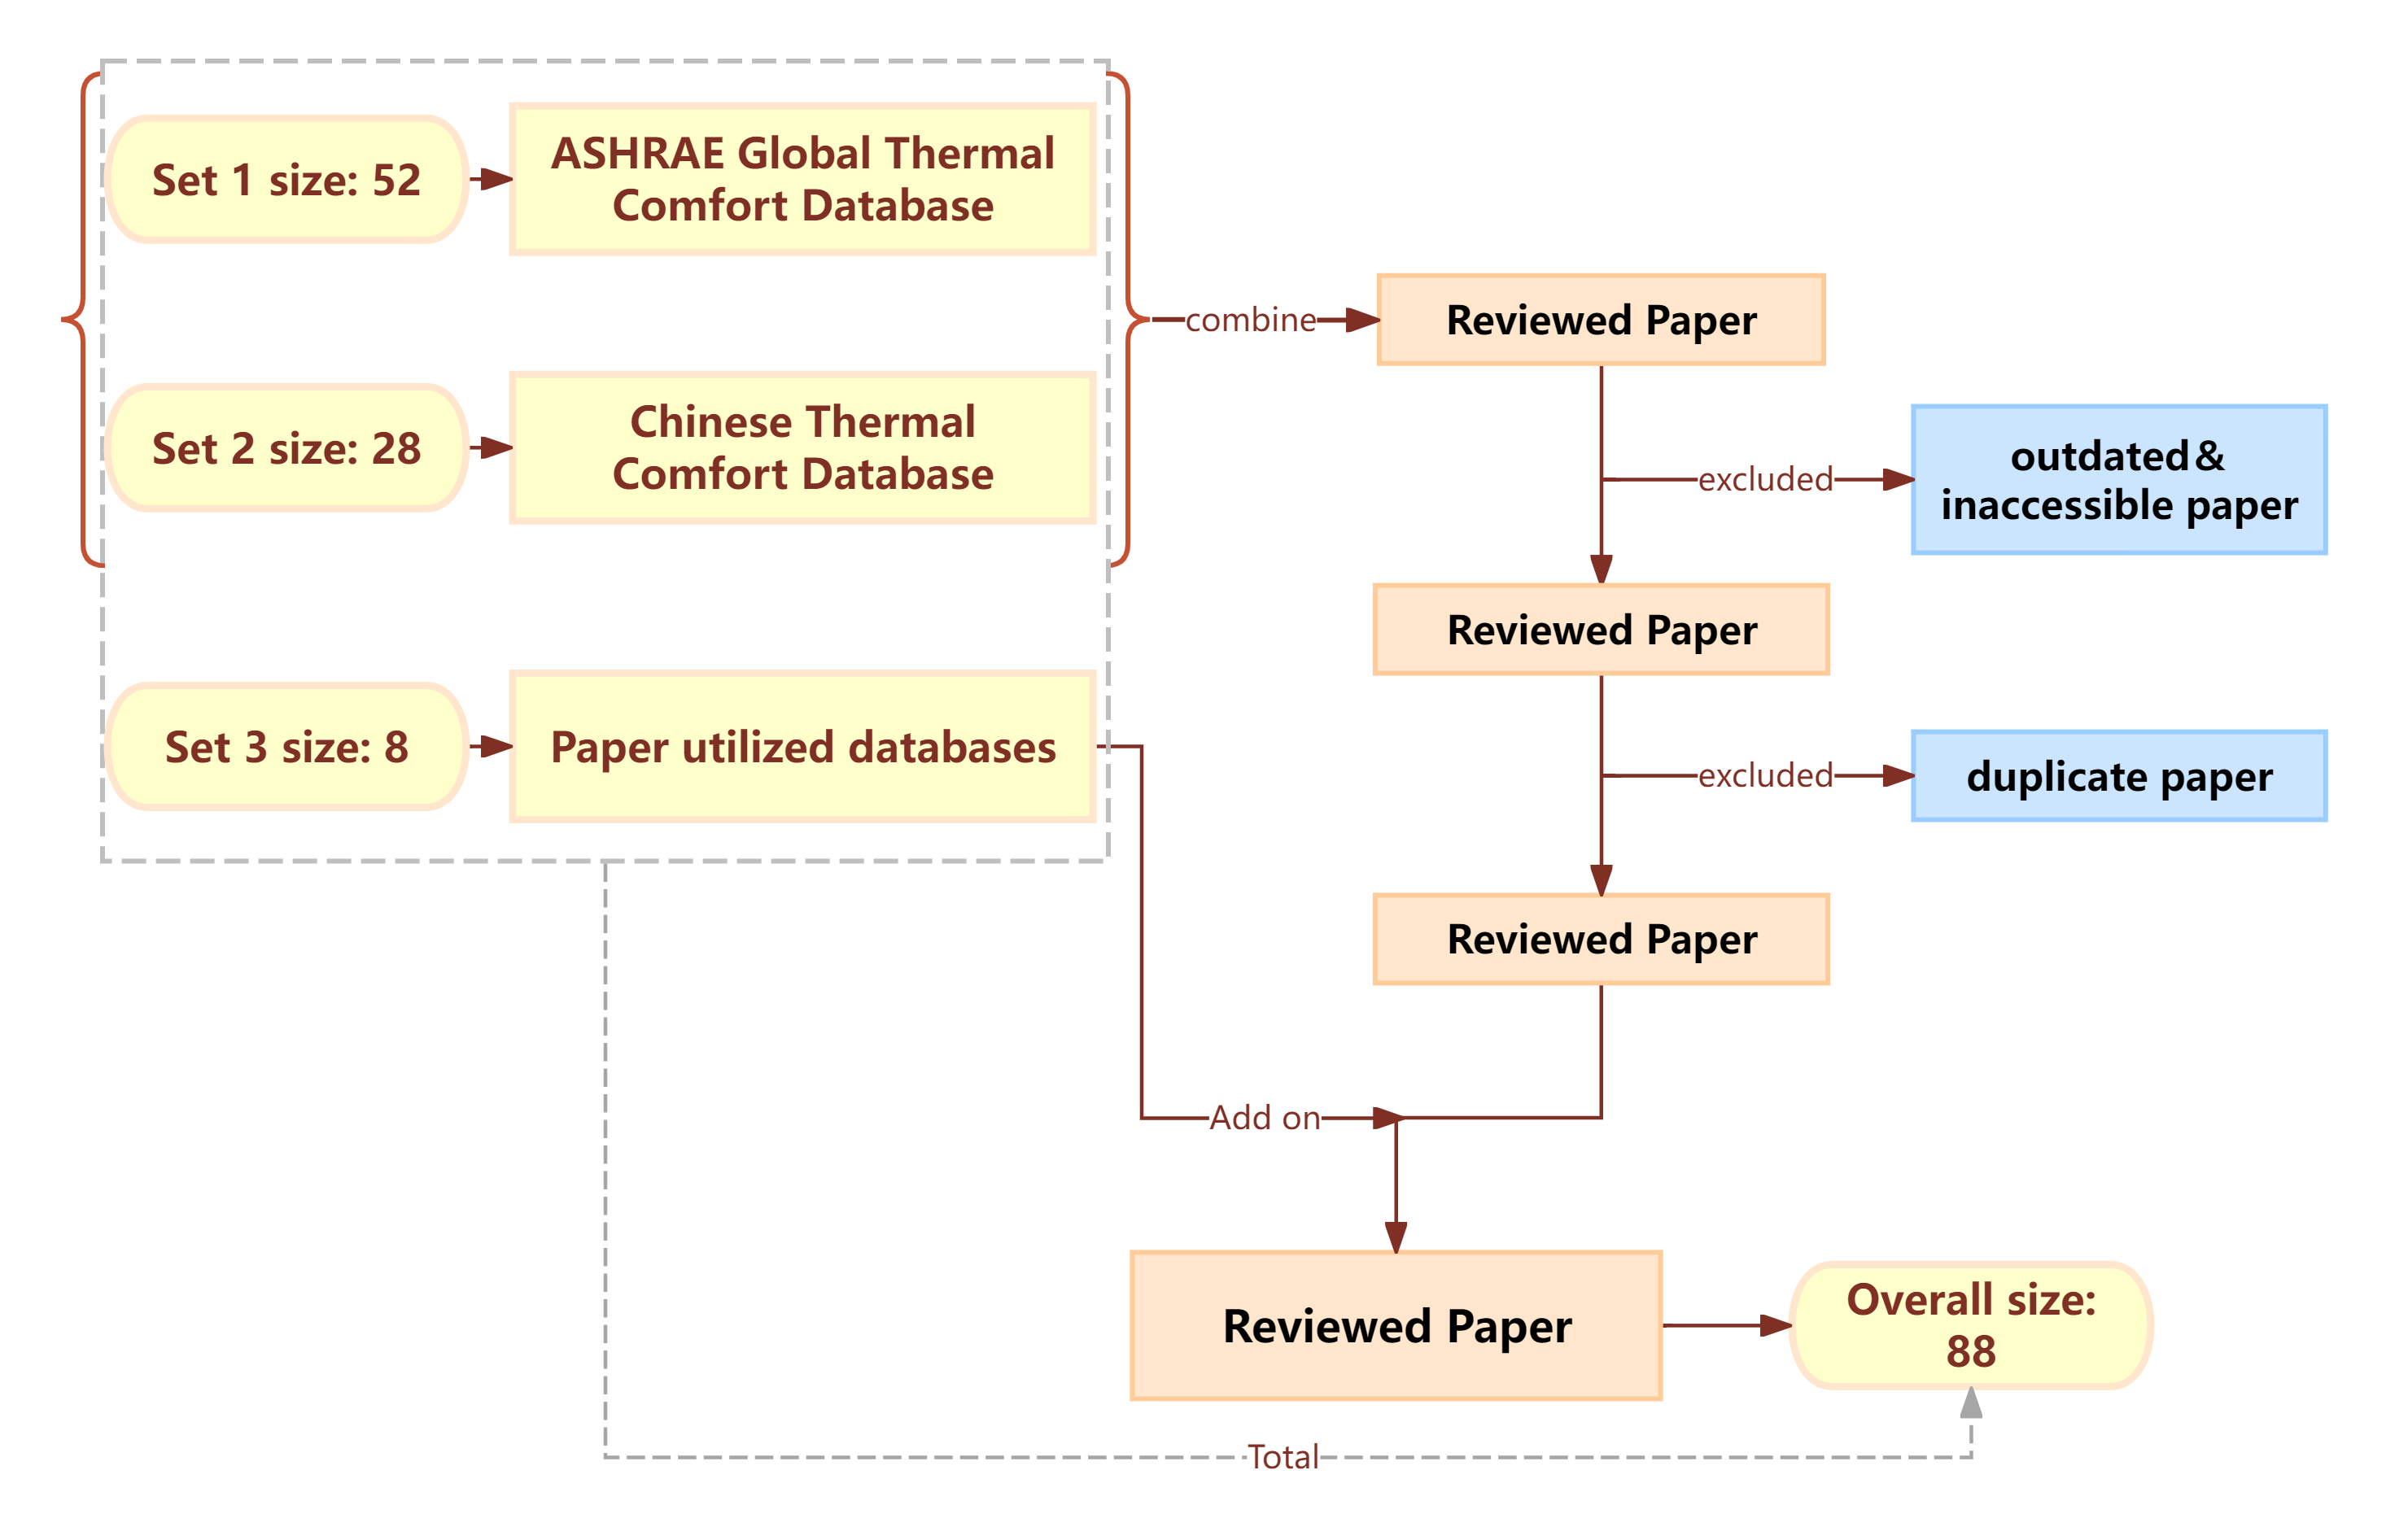
\includegraphics[width=0.85\linewidth]{ab.png} 
    \caption{Flow chart of the selection of studies}
    \label{2}
\end{figure}

\begin{table}[h!]
\centering
\renewcommand{\arraystretch}{1.1} % Adjust row height
\setlength{\tabcolsep}{5pt} % Adjust column spacing
\begin{tabular}{ccc}
\hline
\textbf{Section} & \textbf{Categories} & \textbf{Parameters} \\ \hline
Section A & Basic Information & study ID, dataset, author, year, country, region \\
Section B & Personal Characteristics & age, gender, height, weight, and BMI \\
Section C & Contextual Parameters & climate zones, season, building type, operation mode \\
Section D & Inputs for PMV Calculation & $T_a$, $V_a$, RH, MRT, MET, CLO \\ \hline
\end{tabular}
\caption{Categories in the recording documentation}
\label{table 1}
\end{table}

\subsection{Numerical Evaluation Criteria}
\label{subsec1}

A thorough comparative analysis was conducted to examine the extent to which data collected in each study was utilized. This involved marking whether certain elements were (1) collected and analyzed, (2) collected but not emphasized, or (3) not collected at all. Our evaluation framework draws on data quality classification approaches from two databases. The ASHRAE database \cite{foldvarylicinaDevelopmentASHRAEGlobal2018a} includes a ‘quality assurance’ field for data screening, while the Chinese database \cite{yangChineseThermalComfort2023} classifies data quality into three levels. However, neither database provides a qualitative assessment of individual parameters.

Building upon these approaches, we developed a numerical evaluation system to systematically assess how various parameters were considered across the reviewed studies. Each variable was scored on a scale from 0 to 3, as detailed in Table~\ref{tab:numerical-criteria}. This scale allow us to rate literature based on their level of detail in treating spatial, temporal, and individual variations. A rating of '0' indicates that the parameter is not mentioned at all, either completely absent or without relevant data or analysis. A rating of '1' signifies that the parameter is merely mentioned, with some descriptive categories or statistics provided but lacking in-depth acknowledgment. A '2' rating reflects that the parameter is more thoroughly considered, facilitating comparisons and influencing conclusions about thermal comfort. The '2*' rating is used to denote moderate complexity in variability, whereas a '3' indicates comprehensive consideration with full adaptability across contexts. These distinctions help in systematically assessing the depth of consideration each parameter receives in the reviewed articles. To avoid confusion as the precise definition of numerical values does vary slightly from section to section, we will walk through how we defined values for each of them within the subsequent paragraphs. 

\begin{table}[ht]
\centering
\begin{tabular}{p{5cm} p{10cm}}
\hline
\textbf{Parameter Group} & \textbf{Scoring Criteria (0–3)} \\
\hline
\textbf{Personal Characteristics} & 
\textbf{0}: Not mentioned or not collected \newline
\textbf{1}: Mentioned with minimal stats, no analysis \newline
\textbf{2}: Analyzed, informs thermal comfort discussion \\\hline

\textbf{Contextual Parameters} & 
\textbf{0}: Only single scenario considered \newline
\textbf{1}: Multiple scenarios noted but not analyzed \newline
\textbf{2}: Comparative analysis across categories \\\hline

\textbf{PMV Input Variables} & 
\textbf{0}: Not mentioned \newline
\textbf{1}: Used as constant \newline
\textbf{2}: Used as variable \newline
\textbf{2*}: MRT assumed equal to $T_a$ \newline
\textbf{3}: Vertical gradients considered ($T_a$, RH, $V_a$) \\
\hline
\end{tabular}
\caption{Summary of Numerical Evaluation Criteria for Reviewed Parameters}
\label{tab:numerical-criteria}
\end{table}

 
For personal parameters, numerical ratings between 0, 1, or 2 across five parameters indicate the degree to which each parameter is considered and incorporated in the chosen article. Specifically, ‘0' denotes a lack of consideration for the parameter within the article, either through its complete absence or brief mention devoid of relevant data or analytical findings. It is important to highlight that complete absence encompasses two scenarios. The first scenario is when there is no mention in the article but there is a record in the database, while the second scenario is when there is no mention in either the article or the database. Both instances will be documented as a rating of 0. Transitioning to '1', it signifies a mere mention of the parameter in the article, with varying categories of descriptions or statistics provided but lacking in-depth analysis and conclusions regarding its impact on thermal comfort. Furthermore, '2' indicates thorough consideration of the parameter within the article, facilitating comparisons and influencing conclusions drawn on thermal comfort.

For contextual parameters, 0, 1, or 2 are used to show how detailed contextual parameters - climate zones, season, building type, operation mode - were characterized and discussed in the article reviewed. Specifically, ‘0' indicates that only a singular situation was addressed in the article concerning a specific contextual parameter. Moreover, '1' signifies that despite the consideration of various scenarios for a particular contextual parameter, there is a lack of analysis between that parameter and thermal comfort indicators within the article. On the contrary, '2' indicates that the article not only explores various scenarios within an contextual parameter, but also delves into discussing and analyzing their relationship with thermal comfort indicators according to categories.

For the last section, or canonical inputs to PMV models, situations are a bit different. Given that the six independent variables serve as input parameters for PMV calculation, their numerical values are typically captured during data-acquisition explicitly as numerical values. Specifically, the variables of air temperature ($T_a$), air velocity ($V_a$), and relative humidity (RH) are commonly obtained through direct measurements, while mean radiant temperature (MRT) is typically determined through analytical calculation \cite{guoSimulationMeasurementAir2020,guoUnderstandingMeanRadiant2020}. Conversely, the parameters of metabolic rate (MET) and clothing insulation (CLO) are generally estimated in accordance with ASHRAE 55-2004 and ISO 7730. Owing to the distinct characteristics of each variable and the vertical gradient of the three measured parameters, there are five different numerical ratings (0, 1, 2, 2*, or 3) for the six parameters in Section D. 

Contrast to previous sections, within the last section of value-assignment from our pipeline, ‘0' signifies that this parameter is not mentioned in PMV calculation within the article. Additionally, '1' indicates that the parameter is treated as a constant rather than a variable in PMV calculation. For example, the metabolic rate is often taken as a constant in numerous articles, such as 58.2 W/m$^2$ \cite{luoExploringDynamicProcess2016,wangThermalResponsesDifferent2011,wangThermalComfortNaturally2010}. In contrast, '2' indicates that the parameter is utilized as a variable in PMV calculation. One point worth noting is that '2*' holds particular significance in relation to mean radiant temperature. Instances exist where the mean radiant temperature is presumed to be equivalent to the air temperature \cite{mouFieldStudyThermal2022,duMethodDeterminingAcceptable2021}. In such scenarios, the variable MRT adopts the identical value as $T_a$, despite being a distinct entity. Furthermore, due to the vertical gradient of air temperature, air velocity, and relative humidity, they are typically observed through measurements taken at multiple heights \cite{yangAdaptiveThermalComfort2020,zhangThermalComfortNaturally2010,zhangThermalComfortBuildings2013}. Consequently, for these three parameters, '3' extends beyond '2' by not only comprehensively addressing the parameter but also accounting for its vertical gradient.

\section{Results and Discussions}
\label{subsec1}

\subsection{Current Application of Thermal Comfort Database }
\label{subsec1}

The current research based on thermal comfort databases is extensive, but the research directions are somewhat limited, generally falling into five categories as shown in Table 2. Initially, there are foundational investigations that center on the databases themselves, scrutinizing the significance of specific factors in relation to occupants' thermal comfort. For instance, Wang et al. delves into the influence of individual factors, building characteristics, and geographical variables on variances in individual thermal comfort \cite{wangRevisitingIndividualGroup2020a}. Meanwhile, Du et al. contrasts the impacts of various air conditioning systems on indoor thermal conditions and comfort levels \cite{duComparisonThermalComfort2022a}. Rupp et al. investigates the impact of clothing insulation on thermal comfort predictions \cite{ruppInvestigatingCurrentTrends2021a}. These studies predominantly highlight the effects of individual factors on human thermal comfort, often neglecting the interactions among multiple factors. 

Subsequently, a growing body of research is focusing on refining the original PMV model and leveraging data from thermal comfort databases to validate these refined PMV models or to compare the strengths, weaknesses, and applicability of different PMV models. For example, Cheung et al. verifies the predictive accuracy of the PMV-PPD thermal comfort model and puts forth a simplified model based solely on air temperature \cite{cheungAnalysisAccuracyPMV2019}. In a similar vein, Li et al. assesses the efficacy of seven enhanced PMV models across four distinct climatic regions, offering insights into the suitability of each model for varying climates \cite{liModifiedPredictedMean2025}. Besides, Niza et al. validates several refined PMV models using data from Brazilian cities, highlighting their performance across different climatic conditions \cite{lourenconizaThermalComfortConditions2022}.

\begin{table}[h!]
\centering
\renewcommand{\arraystretch}{1.1} % Adjust row height
\setlength{\tabcolsep}{2pt} % Adjust column spacing
\begin{tabular}{lccc}
\hline
\textbf{Categories} & \textbf{Researcher} & \textbf{Year} & \textbf{Region} \\ \hline
Single-factor influence on thermal comfort & Wang et al.\cite{wangRevisitingIndividualGroup2020a} & 2020 & China \\
& Du et al.\cite{duComparisonThermalComfort2022a} & 2022 & China \\ 
& Rupp et al.\cite{ruppInvestigatingCurrentTrends2021a} & 2021 & Denmark \\ 
Validation and comparison of PMV models & Cheung et al.\cite{cheungAnalysisAccuracyPMV2019}  & 2019 &Singapore \\
& Li et al.\cite{liModifiedPredictedMean2025}  & 2025 & China \\ 
& Niza and Broday\cite{lourenconizaThermalComfortConditions2022}  & 2022 & Brazil \\
& Lamberti\cite{lambertiDevelopmentComparisonAdaptive2023}  & 2023 & Italy \\
& Tartarini and Schiavon\cite{tartariniComparativeAnalysisPMV2025}  & 2025 & Australia \\
Integration with machine learning & Zhou et al. \cite{zhouDatadrivenThermalComfort2020} & 2020 & China\\ 
& Al-Sharif et al. \cite{al-sharifPredictingThermalPreferences2024} & 2024 & Egypt\\
& Nadarajah et al. \cite{nadarajahIdentificationApplicationBestsuited2024} & 2024 & India\\
& Martins et al. \cite{arakawamartinsSystematicReviewPersonal2022} & 2022 & Australia\\
& Haghirad et al. \cite{haghiradAdvancingPersonalThermal2024} & 2024 & Iran\\
& Zhang et al. \cite{zhangAnalysisOutlierDetection2023} & 2023 & China\\
& Wang et al. \cite{wangDimensionAnalysisSubjective2020a} & 2023 & USA\\
& Luo et al. \cite{luoComparingMachineLearning2020c} & 2020 & China\\
Comparison between indoor and outdoor & Hou et al. \cite{houTemporalSpatialHeterogeneity2023} & 2023 & China\\
& Liu et al. \cite{liuComparativeAnalysisIndoor2022a} & 2022 & China\\
Improvements in international design standards & Yang et al. \cite{yangComparativeAnalysisIndoor2024} & 2024 & China\\
& Sun et al.\cite{sunRevisitingAdaptiveThermal2024} & 2024 & China \\
\hline
\end{tabular}
\caption{Selected Thermal Comfort Database usage in categories over the past five years.}
\label{table 2}
\end{table}

While these studies contribute to the refinement of thermal comfort predictions, the practical utility of different models remains constrained and necessitates further enhancement. Recent research has introduced machine learning techniques, which, in contrast to conventional regression analysis, can accommodate a greater number of independent variables without necessitating an exploration of the precise physical interrelationships among each factor. This capability enhances the flexibility and precision of thermal comfort models. For instance, Zhou et al. employed a Support Vector Machine (SVM) algorithm and the RP-884 database to construct a self-learning and self-correcting thermal comfort model \cite{zhouDatadrivenThermalComfort2020}. Similarly, Al-Sharif et al. devised a machine learning predictive model utilizing ensemble algorithms to anticipate occupants' thermal comfort levels \cite{al-sharifPredictingThermalPreferences2024}. Additionally, Nadarajah et al. systematically evaluated ML algorithms like Gradient Boosting and Random Forest for imputing missing thermal comfort parameters, highlighting the importance of algorithm selection based on data characteristics \cite{nadarajahIdentificationApplicationBestsuited2024}. These investigations also propel the advancement of personalized thermal comfort solutions tailored to individual preferences \cite{arakawamartinsSystematicReviewPersonal2022}. 

Furthermore, an increasing number of studies are focusing on the comparative analysis between indoor and outdoor thermal comfort under the growing influence of climate change and urbanization, leveraging thermal comfort databases to uncover distinct patterns in each environment. For example, Liu et al. conducted a large-scale comparative analysis of indoor and outdoor thermal comfort across five climate zones using over 29,000 data points from major thermal comfort databases, revealing that outdoor environments offer a broader comfort range and lower thermal sensitivity compared to indoors \cite{liuComparativeAnalysisIndoor2022a}. Hou et al., using global datasets including the ASHRAE and Chinese Thermal Comfort Databases, found that the relationship between indoor and outdoor temperatures is highly variable, underscoring the need to treat indoor and outdoor comfort separately in health and comfort studies \cite{houTemporalSpatialHeterogeneity2023}. 

Lastly, the existence of various international design standards has raised questions regarding their applicability to thermal environments in diverse countries and regions \cite{bemaInvestigationASHRAEGlobal2023,lourenconizaThermalComfortConditions2022}. To address these concerns, different thermal comfort databases are being leveraged. Yang et al. advocated for revisions to Chinese thermal comfort standards based on ASHRAE RP-884 and a domestic thermal comfort database, culminating in an adaptive thermal comfort model customized for the Chinese populace \cite{yangComparativeAnalysisIndoor2024}. Likewise, Sun recommended adjustments to ISO 17772-1:2017 by drawing insights from diverse databases, leading to the establishment of adaptive models and corresponding adaptive thermal comfort zones \cite{sunRevisitingAdaptiveThermal2024}.

These investigations play a pivotal role in the progression of building technologies and the enactment of energy efficiency policies. Consequently, emphasis should be placed on the regional, cultural, and individual distinctions elucidated by data sourced from various databases. Nevertheless, given that these databases have been curated over a substantial timeframe, the temporal dimension should also be factored into comparative analyses.

\subsection{Visualization of Evaluation Results}
\label{subsec1}

According to the evaluation approach introduced in the previous, the final evaluation results have been shown in the heatmap (Figure~\ref{fig:heatmap_overall}). The color blocks transition from black to light orange, representing ratings from 0 to 3. Specifically, a rating of 0 is depicted as black, a rating of 1 appears as purple, a rating of 2 is represented in red, and a rating of 3 is shown as a light orange. The results of the three sections reveal that the parameters in the Personal Characteristics section receive the least focus among the three, primarily indicated by black blocks. Moreover, the parameters in Section C rank in the middle, with an almost equal distribution of red and black blocks. In contrast, the parameters in the Input for PMV Calculation section received the most attention across all the examined articles, evidenced by a predominance of red blocks, interspersed with black, purple, and light orange blocks in the heatmap.

Transitioning to the distinct sections, we firstly focus on personal characteristics. Among the five parameters within the Personal Characteristics section, the outcomes for age and gender are predominantly represented by purple, with additional occurrences of red and black. This suggests that the reviewed articles mainly offer diverse categories of descriptions or statistics for these two parameters but lack in-depth analysis and conclusive insights on their influence on thermal comfort. Conversely, the visualization results for the parameters height, weight, and BMI are primarily depicted in black, indicating a lack of attention given to these three parameters within the articles. It is worth noting that red blocks are less likely to appear in the heatmap results for personal characteristics. This observation highlights the absence of consideration for the impact of individual variances on thermal comfort analysis within the reviewed articles on thermal comfort data acquisition. 

\begin{figure}[h!]
    \centering
    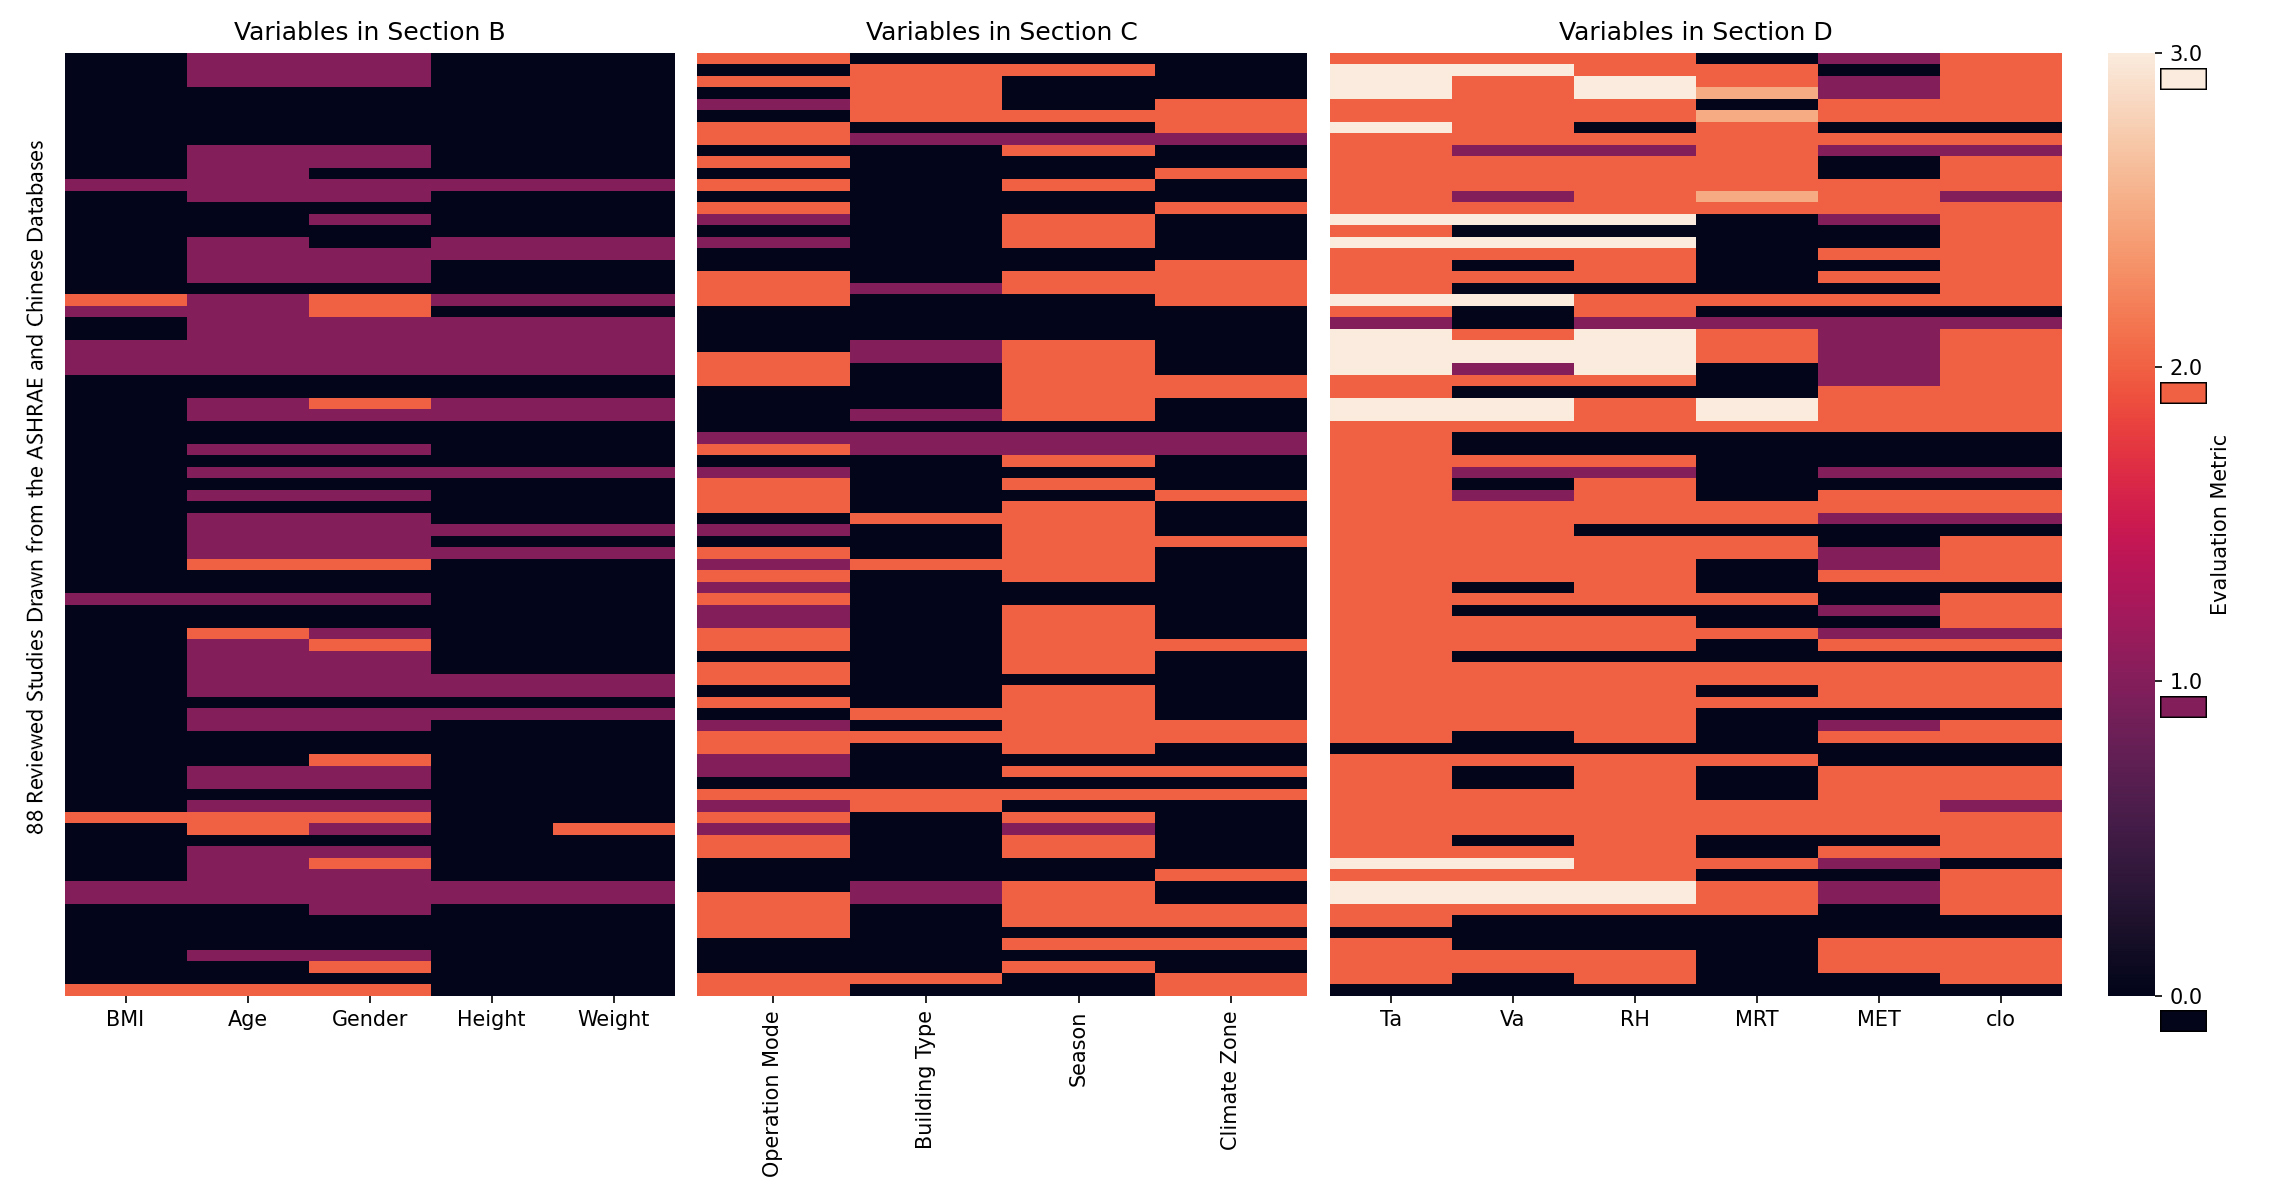
\includegraphics[width=\linewidth]{Heatmap_All_new.jpg}
    \caption{Heatmap for evaluation results of the 88 reviewed studies drawn from the ASHRAE and Chinese Databases, where black, purple and orange corresponds to 0,1 and 2 and the lightest color beige points to 3, increasing respectively on level of details investigated.}
    \label{fig:heatmap_overall}
\end{figure}

Moving onward to the Contextual Parameters section, the heatmap findings can be broadly classified into two distinct categories. The first category encompasses two parameters, namely climate zone and building type, wherein the predominant color is black with supplementary accents of red. This result suggests that the analysis and exploration of thermal comfort across varying categories of these two parameters are insufficient and warrant further investigation. The second category comprises two parameters, season and operation mode, where the primary color is red complemented by black hues. This finding illustrates that many studies have been conducted to discuss and analyze their relationship with thermal comfort indicators according to categories. Furthermore, of the six parameters incorporated into the PMV model, $T_a$, $V_a$, and RH are utilized as variables in the thermal comfort correlation analysis for PMV calculation. The heatmap results mainly feature red blocks with intermittent light orange blocks, signifying the consideration for their vertical gradient. Similarly, the results for CLO are largely represented by red blocks, interspersed with occasional black and purple blocks, indicating a considerable focus on the types and variations of clothing worn by subjects in the literature. In contrast, the heatmap results for MET and MRT exhibit a greater prevalence of black color blocks, suggesting a current inadequacy in the consideration of these parameters in PMV calculations.

\subsection{Evolution of thermal comfort studies over time}

On top of characterizing these parameters individually with respect to their representation across studies as shown in Figure~\ref{fig:heatmap_overall}, we further analyzed trends over time by evaluating the pairwise Pearson correlation coefficients of variables across Sections B, C, and D, as visualized in Figure~\ref{fig:heatmap_corr}. These correlations, derived from the set of 88 thermal comfort studies, allow us to explore evolving research emphases and the stability of variable relationships across years. With reference to \cite{nadarajahIdentificationApplicationBestsuited2024}, we also plotted a complete correlation matrix for selected parameters, which can be found in Appendix with Figure~\ref{correlation}.

\begin{figure}[h!]
    \centering
    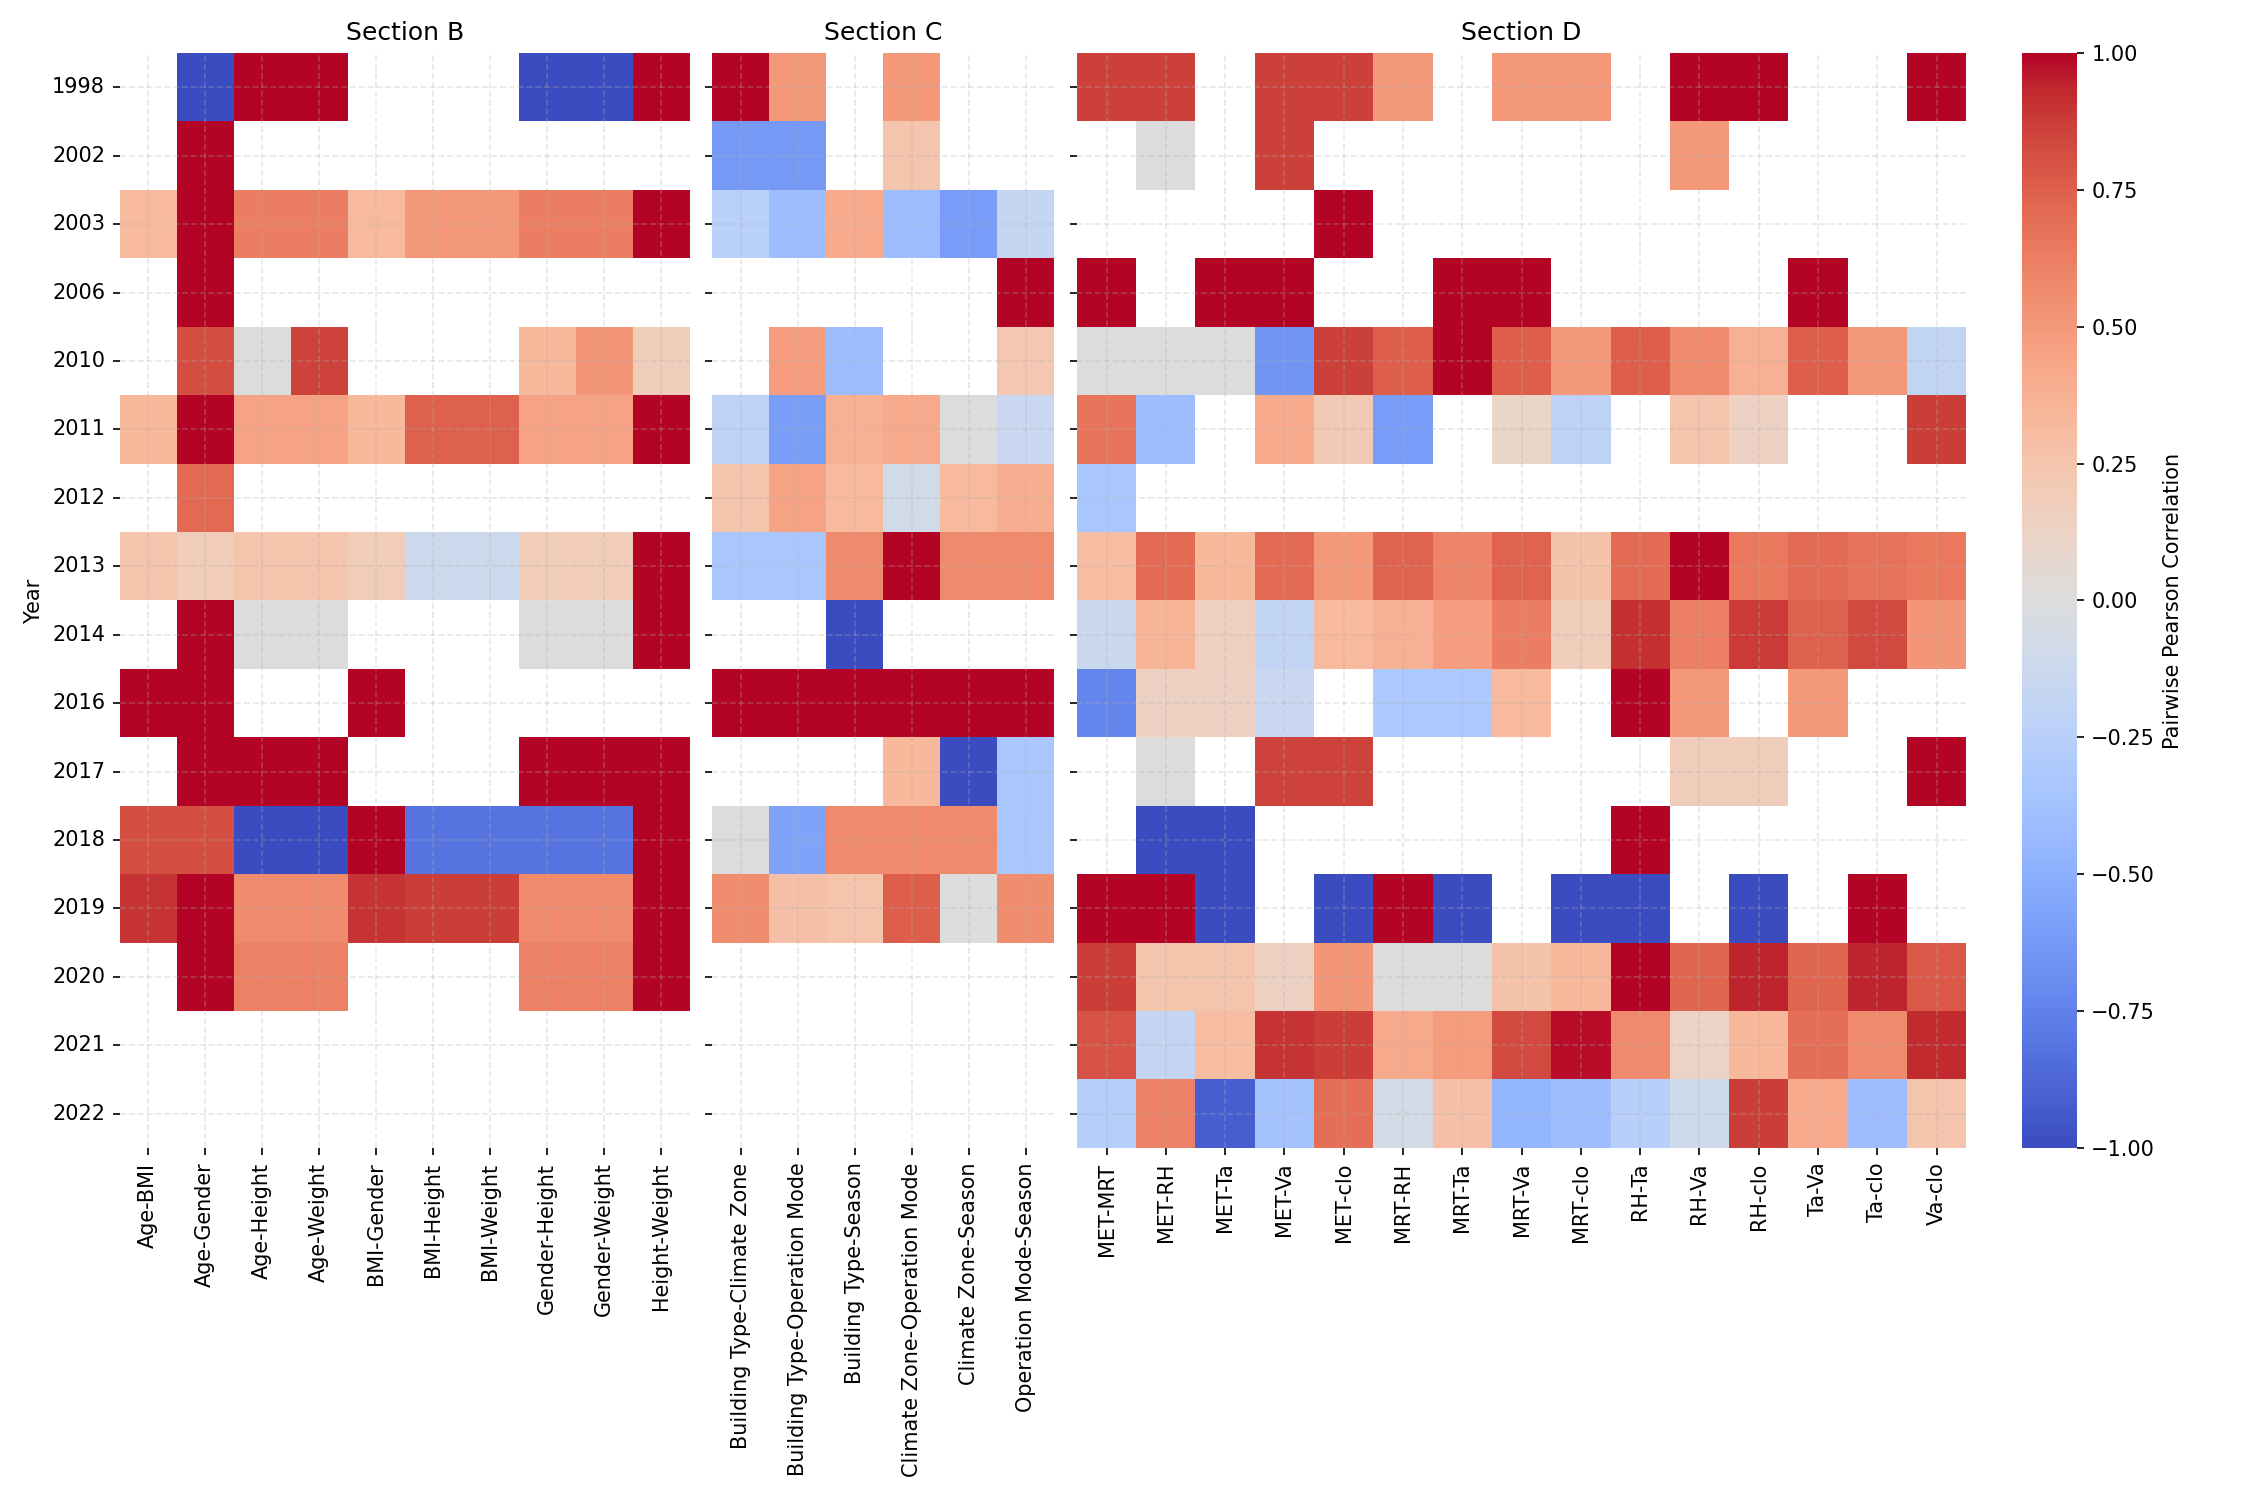
\includegraphics[width=\linewidth]{Heatmap_yearcorr.png}
    \caption{Heatmap for Pearson Correlation Coefficient between paired variables over time across three fields of comparison}
    \label{fig:heatmap_corr}
\end{figure}

Pearson Correlation is a statistical measure that quantifies the linear relationship between two variables. It ranges from -1 to +1, where -1 indicates a perfect negative correlation (one variable increases, the other decreases), +1 indicates a perfect positive correlation (the two variables increase/decrease simultaneously in the same direction), and 0 indicates no linear correlation. This metric helps us to understand how pairwise variables from each of the individual sections are related to each other and how these relationships have evolved over time.

The comparison led to some unsurprising findings across the three different sections. For Section B, two consistently strong variable pairs emerge: 'Age-Gender' and 'Height-Weight'. These recurring correlations showed consistent interests in investigating the two pairs of variables with comparable amount of interests in capturing their details. They can therefore be considered as two 'cores' within Section B, which can be loosely defined as being physique-centric and demographic-centric. Conversely, cross-core relationships such as 'Gender-Weight' or 'Age-Height' show weaker or inconsistent correlations, indicating limited joint exploration in the literature.

Unlike Section B where stable 'cores' pairings emerge, Section C is characterized by more transient and episodically emphasized variable relationships. For instance, the variable pairs 'Building Type–Climate Zone' and 'Building Type–Operation Mode' show moderate to strong positive correlations (in red) in several years, particularly in 2012 and 2016. However, these correlations diminish or even disappear in certain other years, such as 2018 and 2019, potentially indicating that these variable combinations were either deprioritized or integrated into more nuanced research frameworks. Similarly, the correlations between 'Climate Zone–Operation Mode' and 'Operation Mode–Season' display substantial year-to-year variability. For example, these pairs demonstrate weaker associations before 2012 but exhibit significantly stronger correlations in 2016. This fluctuation may suggest increased attention during that period to how climate zones and seasonal changes influence building operation strategies, possibly in response to growing interest in energy-saving practices or climate-adaptive design.

Furthermore, section D also reveals greater variability in correlation strength and direction, particularly for 'MET' with 'RH', '$T_a$', and '$V_a$'. MET's pairwise correlation jumps between strongly correlated and negatively correlated across three important inputs to the PMV models that are also commonly referred to as the most investigated environmental parameters within the indoor environments. These fluctuations suggest researchers continues to be on the fence about how detailed should MET variations be considered across the test subject demographic and over time. Similarly, 'MRT' correlations with other variables also shift from positive (red) to negative (blue) in recent years. These trends may reflect evolving measurement techniques, such as wearable sensors, or shifts in theoretical insights that influence how these variables are captured and analyzed.

Despite these fluctuations, some variable pairs demonstrate persistent and strengthening correlations, such as 'Height-Weight' as well as 'Age-Gender' Pair in Section B, and '$T_a$-$V_a$' pair in Section D. The steady strengthening of this correlation over time could be attributed to increasing emphasis on occupant-centric design and development of more sophisticated sensing and logging systems where air temperature and velocity can be better analyzed and captured. These steady relationships points to certain aspects of thermal comfort research maintaining good momentum and moving in well-established directions. 

These findings underscore the existence of both stable and shifting research priorities in thermal comfort research. While steady correlations suggest mature areas of study, variable or weakening trends highlight areas of theoretical reconsideration or methodological evolution. These patterns help identify core influences on thermal comfort and reveal potential research gaps where variable pairings are underexplored or increasingly divergent.

While we believe results presented in Figure~\ref{fig:heatmap_corr} provides valuable insights into how data-driven thermal comfort studies have evolved over the years, it's also important to acknowledge the limitation of our current approach. One clear limitation is the selection of the 88 papers included in the analysis. Although the papers were carefully hand-picked based on their relevance to thermal comfort research and contribution to thermal comfort databases, other relevant studies could have been included, which could potentially influence the observed trends and correlations. On top of that, the categorization and assignment of numerical values to the variables in each paper involved some level of subjectivity. While efforts were made to ensure consistency and reliability in the coding process, there may be some inherent variability and bias built in on how the authors chose to report their findings in their manuscripts. Another clear limitation is how the number of papers may have changed over years, the more recent the studies become, the more data-rich each of the heat map pixel becomes, nonetheless there are still cases where there are no values, pointing to potentially future work if this approach gets implemented by other authors who are interested in expanding this to be more inclusive of additional literature. 

% Pearson Correlation is a statistical measure that quantifies the linear relationship between two variables. It ranges from -1 to +1, where -1 indicates a perfect negative correlation (one variable increases, the other decreases), +1 indicates a perfect positive correlation (the two variables increase/decrease simultaneously in the same direction), and 0 indicates no linear correlation. Within the scope of our current investigation, Pearson Correlation helps us to understand how pairwise variables from each of the individual sections are related to each other and how these relationships have evolved over time.

% This comparison led to some unsurprising findings across the three different sections. For Section B, there appears to be two consistent groups of pairwise variables, i.e. 'Age-Gender' and 'Height-Weight'. This indicates that the studies that occurred within our span of investigation showed consistent interests in investigating the two pairs of variables with comparable amount of interests in capturing their details. They can therefore be considered as two 'cores' within Section B, which can be loosely defined as being physique-centric and demographic-centric. Investigations that happens across the two cores, e.g. correlation between 'Gender-Weight' or 'Age-Heght' appears to have received much less if not no joined attention within the set of literature we identified. 

% Section D exhibits more variation in directional change of pairwise correlations, particularly between "MET-RH" , "MET-Ta" and "MET-Va." MET's pairwise correlation jumps between strongly correlated and negatively correlated across three important inputs to the PMV models that are also commonly referred to as the most investigated environmental parameters within the indoor environments. This could mean researchers continues to be on the fence about how detailed should MET variations be considered across the test subject demographic and over time. This is also true for MRT whose pairwise correlation with RH, Ta and Va as well as CLO saw their values flipping from positive to negative within the most recent studies. These weakening correlations in recent years (shifting from red to blue) may indicate a change in how researchers perceive the relationship between metabolic rate, mean radiant temperature and the rest of the inputs to PMV models. This shift could be attributed to advancements in measurement techniques such as wearable sensors and additional insights that do not get captured by the analyzed variables, leading to a recent change in their interactions.

% Nonetheless, there are consistent changes in pairwise correlation overtime, where certain pairs of variables exhibited consistent shifts in how detailed their respective investigation are throughout the years they were published. These steady relationships points to certain aspects of thermal comfort research maintaining good momentum and moving in well-established directions. Examples like this could be found in the 'Height-Weight' as well as 'Age-Gender' Pair in Section B, and 'Ta-Va' pair in Section D, suggesting that researchers have consistently considered the influence of the pair on thermal comfort perception. The steady strengthening of this correlation over time could be attributed to increasing emphasis on occupant-centric design and development of more sophisticated sensing and logging systems where air temperature and velocity can be better analyzed and captured.

% These consistent trends across variable pairs highlights the presence of well-established relationships in recognizing variables used by thermal comfort research as seen through the thermal comfort databases. While identifying these steady relationships, we could gain insight into the core factors that are more recently investigated that is believed to be influencing thermal comfort perception and identify potential research gaps when recent studies starts to deviate from as well as voids left in these recent studies thereof.

% While we believe results presented in Figure~\ref{fig:heatmap_corr} provides valuable insights into how data-driven thermal comfort studies have evolved over the years, it's also important to acknowledge the limitation of our current approach. One clear limitation is the selection of the 88 papers included in the analysis. Although the papers were carefully hand-picked based on their relevance to thermal comfort research and contribution to thermal comfort databases, other relevant studies could have been included, which could potentially influence the observed trends and correlations. On top of that, the categorization and assignment of numerical values to the variables in each paper involved some level of subjectivity. While efforts were made to ensure consistency and reliability in the coding process, there may be some inherent variability and bias built in on how the authors chose to report their findings in their manuscripts. Another clear limitation is how the number of papers may have changed over years, the more recent the studies become, the more data-rich each of the heat map pixel becomes, nonetheless there are still cases where there are no values, pointing to potentially future work if this approach gets implemented by other authors who are interested in expanding this to be more inclusive of additional literature. 

% Moreover, we also conduct the correlation between these variables, which has been shown in Figure~\ref{fig:heatmap_corr}. The color blocks exhibit a gradient shift from blue to red, denoting correlations ranging from disparate to congruent. More precisely, when two variables exhibit inverse trends simultaneously, they are visualized as blue. In the absence of correlation between the two variables in a given year, a grey block is utilized. Conversely, when both variables demonstrate synchronous directional alignment and magnitude, they are depicted in red. 

% In terms of the research year, variables within the three categories have been involved in thermal comfort-related studies since approximately 2000, with an increase in the volume of scholarly articles and a deepening of research efforts over the past decade. Regarding the overall research tendency, investigations into the interplay among the five variables of personal characteristics have witnessed rapid development in the last decade, characterized by a robust correlation primarily indicated by red color blocks. Conversely, research on the correlation among the four variables of contextual parameters has exhibited a lower level of association, predominantly represented by blue color blocks, although some improvement in correlation was observed in 2019. The relationship among the six variables related to PMV calculation inputs has demonstrated greater variability, with a stronger correlation evident around 2000, followed by a gradual weakening of correlations from 2000 to 2015, and an increase in opposing correlations among the variables in more recent years.

\subsection{Personal Characteristics}
\label{subsec1}

As shown in Figure~\ref{fig:heatmap_overall}, the five parameters - age, gender, height, weight, and Body Mass Index (BMI) - pertaining to personal characteristics outlined in Section B are not fully considered in the analysis of thermal comfort, predominantly represented by numerical ratings of 0 or 1.

\subsubsection{Age}

The first parameter we examined is age. The results show that 61.0\% of the reviewed articles considered age as a variable in data collection and subsequent subject analysis. 
Most articles leveraged limited data-processing methods for age, such as reporting overall age ranges \cite{zhouThermalComfortRadiant2019,zhouRadiantAsymmetricThermal2022}, analyzing summary statistics \cite{caoIndividualDistrictHeating2014,caoTooColdToo2016,wangThermalAdaptationThermal2014,wangIndividualDifferenceThermal2018,yanAnalysisBehaviourPatterns2016,yanInfluenceOutdoorTemperature2016}, or listing individual ages \cite{xuEnvironmentalFactorsAffecting2021} without grouping subjects.
These approaches resulted in the lack of comparative analysis of thermal comfort indicators between various age groups in the research. 
Among articles that categorized subjects into age groups, the bins used for age groupings also varied across studies, likely due to the wide range of ages represented.
For instance, some studies \cite{boudenAdaptiveThermalComfort2005,jiaThermalComfortMixedmode2020,konisEvaluatingDaylightingEffectiveness2013} segmented subjects' ages in 10-year intervals, while others adopted the flexible grouping approach \cite{wangRevisitingIndividualGroup2020b,singhRelationIndoorThermal2014}, such as two groups in 10-20 and 20-40, three groups in below 20, 20-40, and above 40 \cite{singhThermalPerformanceStudy2010}. 
These findings highlight a clear lack of universally accepted standard for age groupings in global thermal comfort surveys, which hinders comparative analysis across different studies, let alone different databases.
Furthermore, the results also indicate that the age range of the subjects in the reviewed studies was primarily concentrated between 18-25 years old, lacking the composition of data from older adults and children.

In the articles with full consideration of the age parameter, while all these articles established a connection between the age parameter and analyses related to thermal comfort, there is a notable discrepancy in the depth of analysis. Among them, three articles with a weaker association \cite{honnekeriComfortAdaptationMixedmode,tartariniThermalPerceptionsPreferences2018,vecchiThermalHistoryIts} only examined aspects such as the distribution of subjects' ages across different building operation modes and the relationship between age and clothing insulation. Their analysis and conclusions did not point out variations in thermal comfort-related indicators among different age groups. In contrast in the articles with a stronger association, Zhe Wang \cite{wangRevisitingIndividualGroup2020b} focused on the differences between age as well as neutral temperature and thermal sensitivity. The results showed that in the age range of 10 to 40 years old for which data are predominant, teenagers have a higher neutral temperature and could tolerate a wider temperature variation compared to adults. Despoina Teli \cite{teliNaturallyVentilatedClassrooms2012} argued that the current thermal comfort models, which was built based on adults, were not appropriate for children. His study showed that children are inclined to a warmer thermal sensation and a colder indoor thermal environment than adults. In future research, it is recommended that a more comprehensive comparison be conducted among different age cohorts across thermal comfort indicators. For instance, in the article authored by Madhavi Indraganti which is not included in both of the databases \cite{indragantiEffectAgeGender2010}, he compared the differences between two age groups (over 40 years old and under 40 years old): thermal sensation, thermal preference, thermal acceptance, and overall comfort. The study findings suggested that older individuals displayed greater tolerance towards variations in the thermal environment.

\begin{figure}[h!]
    \centering
    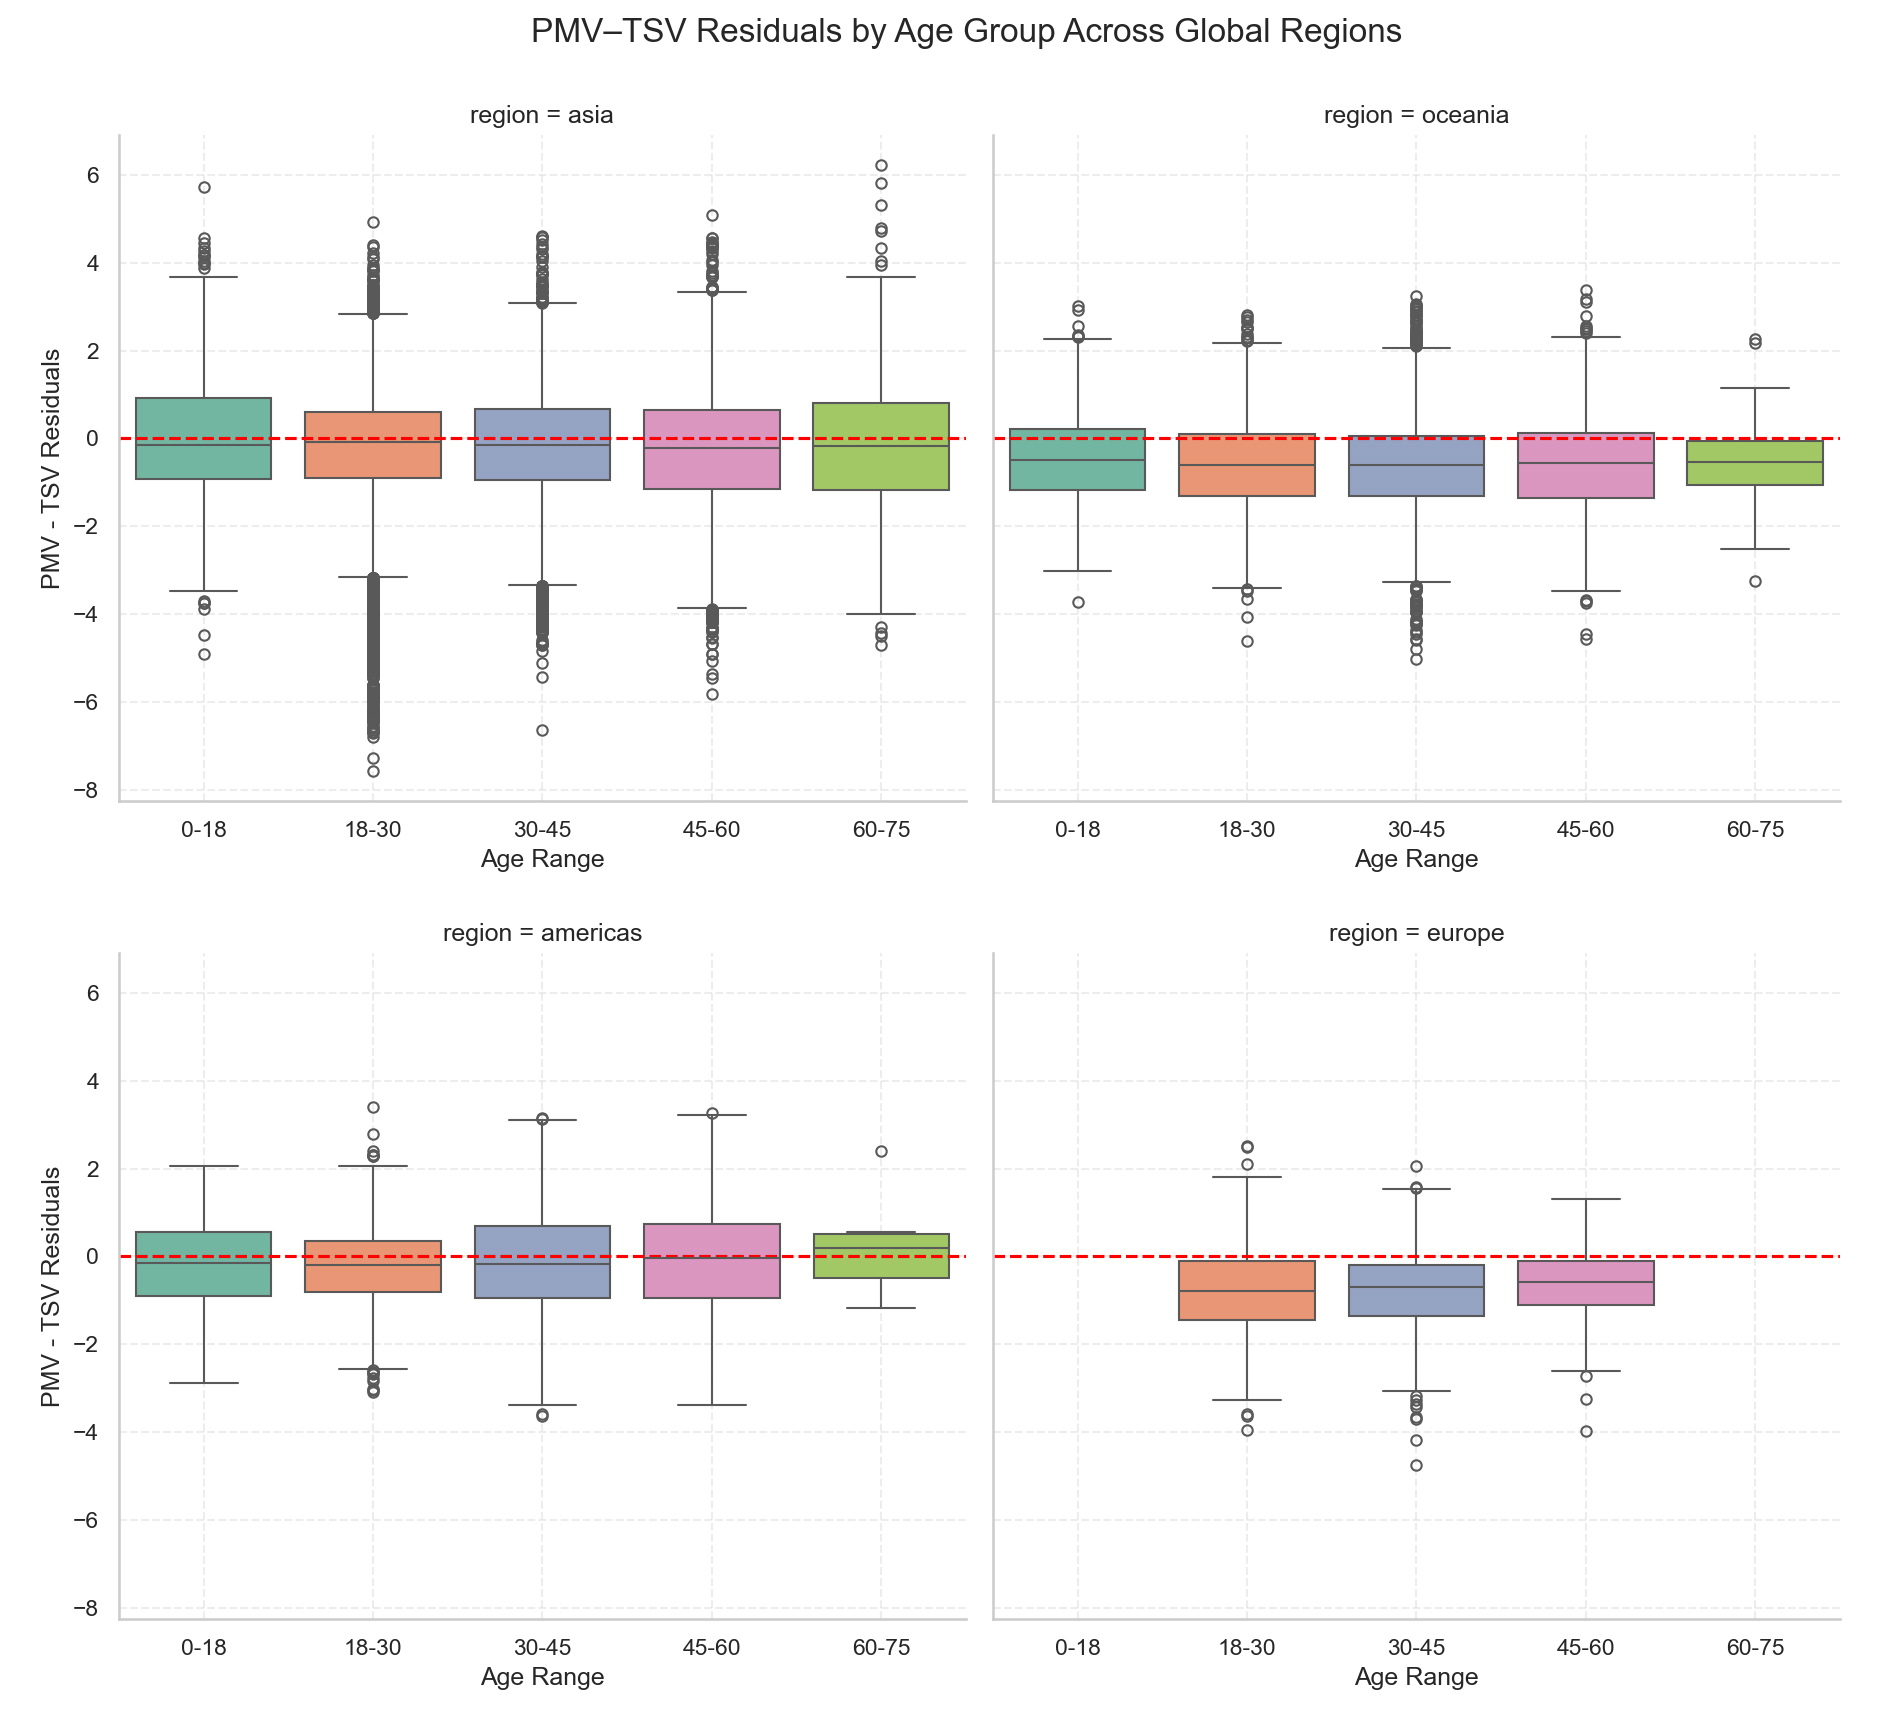
\includegraphics[width=0.8\linewidth]{facet_age_residuals_new.jpg}
    \caption{Box plot of the differences between PMV and TSV across age with respect to different regions}
    \label{5}
\end{figure}

The Box plot of the differences between PMV and TSV across age with respect to different regions is shown in Figure~\ref{5}. In terms of data availability, age data were systematically gathered for Australian, American, and Asian participants, encompassing a broad spectrum of age cohorts. Conversely, the demographic profile of European subjects is predominantly centered within the 18-60 age bracket, with gaps in data pertaining to children, adolescents, and older adults. In contrast, the availability of age-related data for subjects from Africa is limited. In relation to the overall results, the measures of central tendency for the residuals (TSV-PMV) in the Americas and Asia closely approach zero, while those in Oceania and Europe register below zero. Additionally, the residual distribution is more concentrated in the Americas and Europe, in contrast to Asia where it exhibits more fluctuation. Ultimately, the data from the Americas exhibited the most precise predictions of PMV values within each age grouping, with minimal error fluctuations.

Transitioning to the distinct regions, we firstly focus on Oceania. The median discrepancy between the residuals of PMV and TSV across the five age categories is relatively minor, falling within the range of approximately -0.5 to -1.0, with 75\% of the data distributed below zero. Moreover, the least significant variations in residuals were observed within the older age bracket (aged 60-75), while the greatest fluctuations were evident in the middle-aged cohort (age 30-60). This observation implies that predictive accuracy of PMV values is more reliable among older individuals compared to the younger counterparts in Australia. Moving onward to the Americas, in relation to the measures of central tendency for the residuals, the age groups of 18-30 and 45-60 exhibit a tendency towards zero, whereas the central tendency of the remaining three age groups demonstrates fluctuations both above and below zero. Regarding the data distribution, the residuals associated with the 60-75 age group display a more centralized distribution with a narrower range of variability, contrasting with the more dispersed distribution and wider range of variability observed in the three age groups spanning 18-60. These findings imply that older individuals in the Americas represent a more reliable age cohort for predicting PMV values.

For the three age groups in Europe, the median values of the residuals fall within the range of -1.5 to -0.5, with the interquartile range indicating that the middle 50\% of the data lies below zero across all three age groups. Regarding variability, the residuals for the 45-60 age group exhibit minimal fluctuation, ranging from -3 to 3, in contrast to the wider fluctuation range of approximately -4 to 4 observed in the age groups of 18-30 and 30-45 years. Overall, the 45-60 age group demonstrates better predictive accuracy of PMV values within this dataset. When we examined the results in Asia, the measures of central tendency for the residuals in all five age groups tend to be zero. Except for the elderly group of 60-75 years old, the middle 50\% of the data of the other four age groups show a centrosymmetric distribution. Regarding the variability of the residuals, the elderly group displays the narrowest range of fluctuation, ranging from -4 to 3. This is followed by the age groups of 0-18 years and 45-60 years with a range of approximately -5 to 4, while the two groups spanning ages 18-45 years exhibit the widest range of fluctuation, approximately ranging from -6 to 5.

Combining the age outcomes across the four regions, it can be inferred that PMV does a better job at predicting thermal comfort amongst the age group of 60-75 years compared to the other age cohorts. This conclusion may stem from the older age group being less susceptible to external environmental influences and exhibiting a higher likelihood of maintaining a consistent body temperature and activity level.

\subsubsection{Gender}

Moving onward to the next parameter that we examined, the gender parameter was generally accompanied by the age parameter in the reviewed articles, also presenting similar outcomes. According to the reviewed results, 63.4\% of articles considered age as a variable in data collection and subsequent subject analysis, a bit higher than the results of the age parameter. Among them, a notable observation is that the analysis approach for the gender parameter was typically presented in two main formats. The first involved a brief textual description of gender distribution during subject introduction within the methodology section of the articles \cite{zhouThermalComfortRadiant2019,caoIndividualDistrictHeating2014,manuFieldStudiesThermal2016}. The second entailed a more explicit representation through graphs or tables \cite{boudenAdaptiveThermalComfort2005,caoFieldStudyHuman2011,hawighorstThermospecificSelfefficacySpecSE2016}. 

When examining the articles with full consideration of the gender parameter, there have been a number of studies examining the relationship between gender and clothing insulation \cite{tartariniThermalPerceptionsPreferences2018}, gender and various operation modes \cite{vecchiThermalHistoryIts}, gender and indoor environmental factors affecting sleep quality \cite{xuEnvironmentalFactorsAffecting2021}, gender and the building symptom index (BSI) \cite{sekharIndoorAirQuality2003}. 
While these articles presented investigation on the relationship between gender and various factors related to thermal comfort, they do not provide conclusive evidence on the direct link between gender and thermal comfort indicators.
However, some articles does directly address this relationship.
These researchers pointed out a weak correlation between gender and thermal sensation but a strong correlation between gender and thermal acceptance. Specifically, females showed slightly higher thermal acceptance than males, indicating a preference for warmer environments \cite{wangFieldStudyThermal2006}. Furthermore, research findings indicate that females were more sensitive than males according to temperature variation \cite{wangRevisitingIndividualGroup2020a} and more prone to expressing thermal dissatisfaction than males \cite{dedearFieldExperimentsOccupant}, especially in cold discomforted environments \cite{langevinTrackingHumanbuildingInteraction2015}. 
These findings suggest that gender could be a crucial factor in predicting thermally driven behaviors and should be taken into consideration by thermal comfort models.


\begin{figure}[h!]
    \centering
    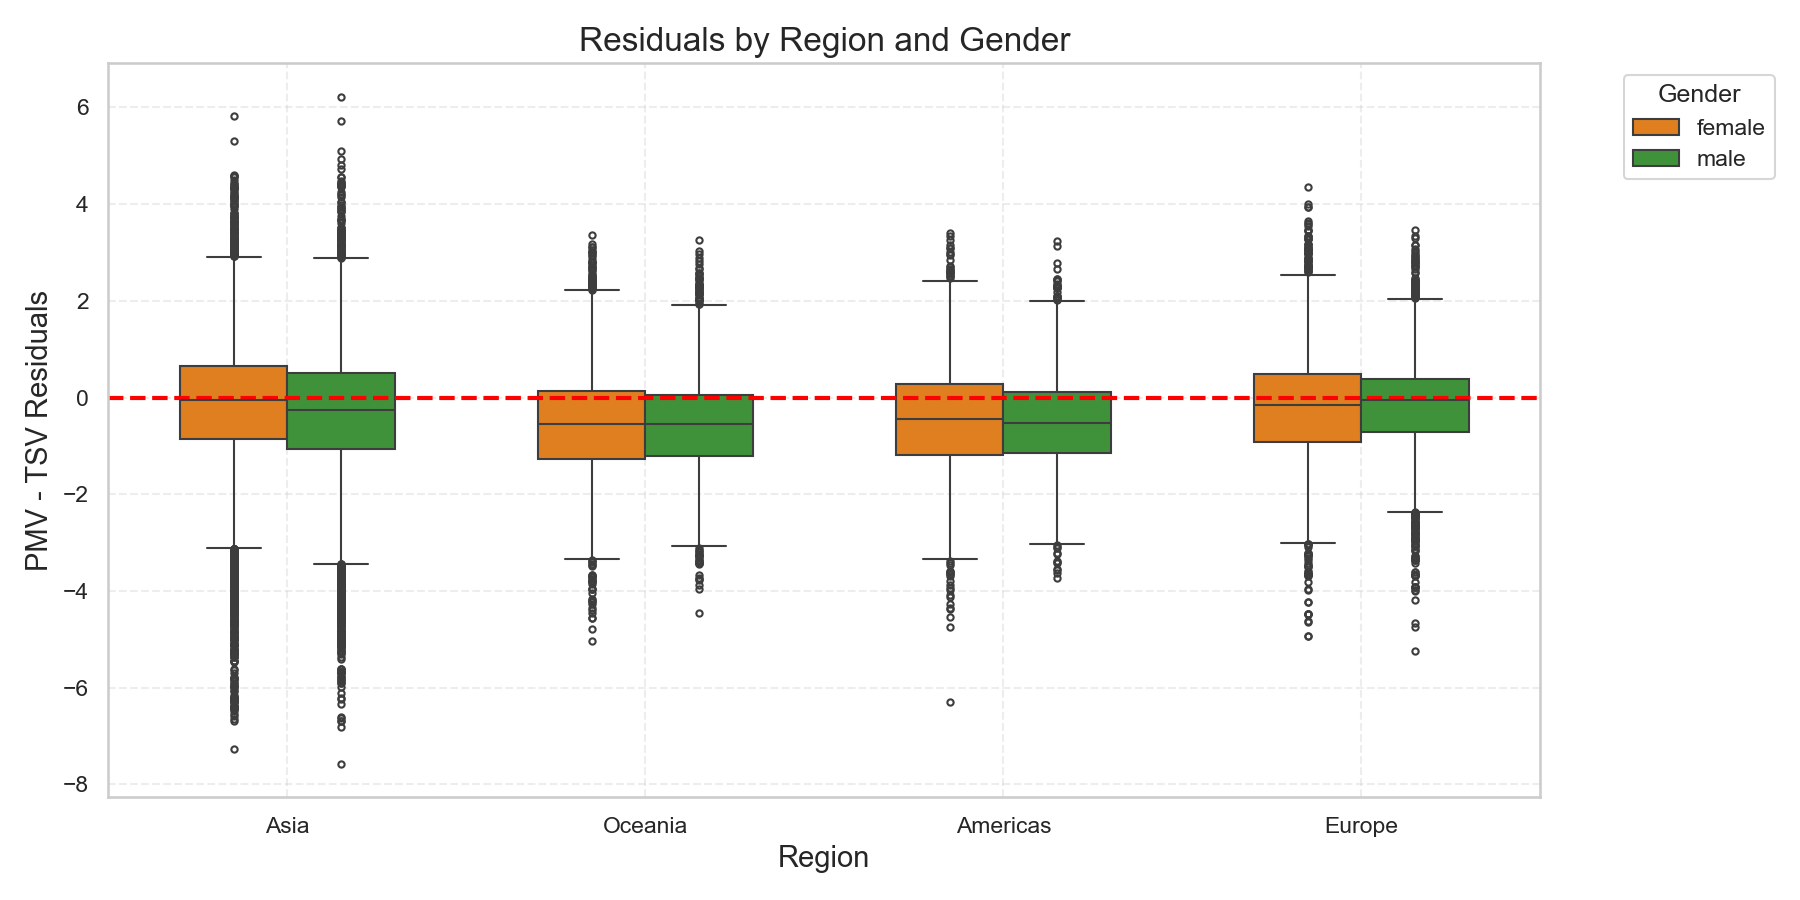
\includegraphics[width=0.9\linewidth]{reg_gen.png}
    \caption{Box plot of the differences between PMV and TSV across gender with respect to different regions}
    \label{6}
\end{figure}

Moving onward to the gender results, Figure~\ref{6} shows the box plot of the differences between PMV and TSV across gender with respect to Oceania, the Americas, Europe, and Asia. Regarding the overall findings, the measures of central tendency for the residuals (TSV-PMV) in Europe and Asia closely approach zero, whereas those in Oceania and the Americas range between -1.0 and -0.5. Analyzing the interquartile range reveals a higher concentration of the middle 50\% of residuals in Europe, while dispersion is more pronounced in Asia. Consequently, the data sourced from Europe emerges as a more dependable source for forecasting PMV values.

When examining the results in Oceania in detail, both male and female groups exhibit similar box plots with median residuals hovering around -0.5 and fluctuations ranging between -5 and 3.5. Transitioning to the results in the Americas, male residuals are more concentrated than females, with a smaller fluctuation range. Furthermore, in Europe, median residuals for both genders are approximately zero, but female residuals show wider fluctuation (around -5 to 5) compared to males (around -4 to 4). Whereas in Asia, both male and female residuals display large fluctuation ranges, with males showing a particularly pronounced range. The measures of central tendency for both genders is around zero, slightly lower for males. The gender results across the four regions shows minimal variation in the box plots between males and females. This suggests that gender as a personal characteristic has negligible impact on the accuracy of PMV values.

\subsubsection{Height, Weight, and BMI}

Different from the review results of age and gender, the two parameters - height and weight have received relatively less attention in all the reviewed articles. Since both parameters in most cases typically appear simultaneously through the data collection and analysis phases, they are combined and analyzed together here. According to the review results, 75.6\% of the articles did not mention subjects’ height and weight information, while one article included in ASHRAE database in which the weight parameter was fully considered and analyzed. This result suggests that the two parameters, height and weight, are inadequately analyzed in the research of thermal comfort. In terms of the analysis method, subjects’ height and weight data was generally presented in tables. Most articles \cite{dedearFieldExperimentsOccupant,kwokThermalComfortJapanese2003,molinaFieldStudyOccupant} computed the maximum, minimum, mean, and standard deviation of both parameters, with a few articles \cite{zhangThermalComfortPeople2020,baePredictingIndoorThermal2017} displaying the range of the two parameters. Conversely, in the article conducting analysis \cite{teliNaturallyVentilatedClassrooms2012}, the research focused on the correlation between weight and metabolic rate, suggesting that children exhibit a higher metabolic rate per kilogram of body weight in comparison to adults.

Based on the analysis of height and weight, we lastly examined the BMI parameter. BMI (Body Mass Index) is a numerical value calculated using a person's weight and height. BMI is commonly used to classify individuals into categories such as underweight, normal weight, overweight, or obese. It has gained more and more focus in the research as an important indicator currently. However, in the field of thermal comfort database, the BMI parameter received even less attention compared to height and weight according to the review results. In all the reviewed articles, 9.8\% of the articles merely mentioned the BMI parameter without in-depth analysis and conclusions regarding its impact on thermal comfort. Researchers only added the participants' BMI information into the questionnaire to collect it without extended analysis. The only difference was reflected in the data presentation methods, such as documenting the precise BMI data of each subject \cite{jiaThermalComfortMixedmode2020}, calculating the mean and standard deviation value \cite{xuEnvironmentalFactorsAffecting2021}, or directly showing the overall range \cite{hawighorstThermospecificSelfefficacySpecSE2016,zhangThermalComfortPeople2020}. 

Whereas in the 3.7\% of the articles with full consideration of the BMI parameter, the analysis was prone to be more specific and in-depth. Federico Tartarini \cite{tartariniThermalPerceptionsPreferences2018} delved into the correlation between variations in clothing insulation and BMI of participants. The study findings suggested that individuals within the normal BMI range exhibited a tendency to wear more clothes than those within the obese BMI range. Zhe Wang \cite{wangRevisitingIndividualGroup2020a} divided the subjects into three groups - underweight, normal, and overweight - according to their BMI data for the purpose of examining and comparing their thermal neutrality and thermal sensitivity. Their research observed that individuals with higher BMI values exhibited a higher sensitivity to thermal variations, a preference for lower temperature environments, and a broader comfort zone. Specifically, Zhe Wang \cite{wangRevisitingIndividualGroup2020a} innovatively concluded for the first time that overweight individuals could tolerate a 60\% wider temperature range than normal subjects.

\begin{figure}[h!]
    \centering
    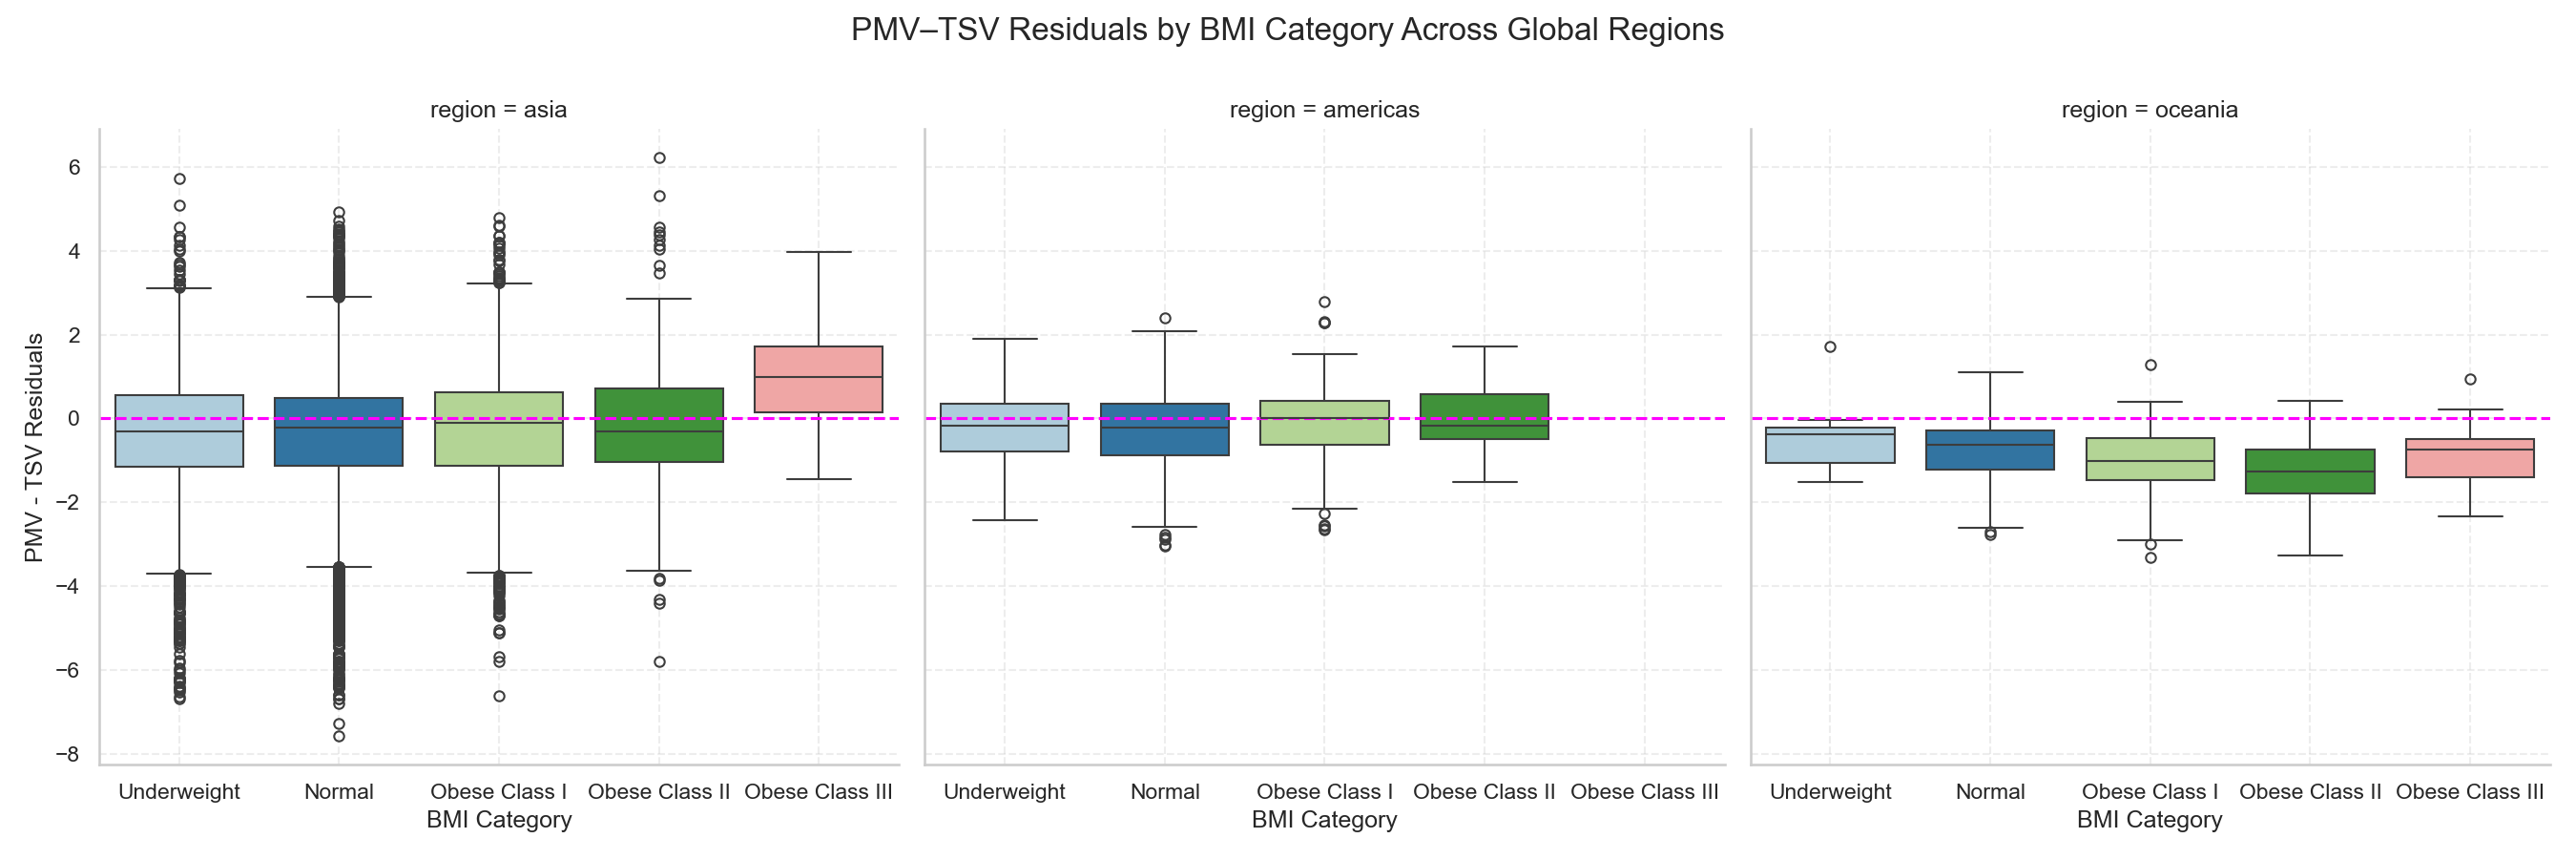
\includegraphics[width=1.0\linewidth]{facet_bmi_residuals_new.png}
    \caption{Box plot of the differences between PMV and TSV across BMI with respect to different regions}
    \label{7}
\end{figure}

Compared to the results of age and gender, a more substantial regional difference was observed for BMI, as depicted in Figure~\ref{7}. BMI data were collected from three regions - the Americas, Australia, and Asia - and categorized into five groups: underweight (0-18.5 kg/m$^2$), normal (18.5-25 kg/m$^2$), Obese Class I (25-29.9 kg/m$^2$), Obese Class II (29.9-35 kg/m$^2$), and Obese Class III (35-40 kg/m$^2$). Analysis of the central tendency of residuals revealed a significant deviation for the BMI groups in Australia and the Obese Class III group in Asia, while other groups tended to approach zero. In terms of interquartile range, the distribution of middle 50\% of the data in Australia was the most concentrated with a range of approximately 1, followed by the Americas with a range of about 1.5, and Asia exhibited the most discrete data with a range of around 2. The overall fluctuation of residuals indicated a smaller range between -3 and 2 for the Americas and Australia, while Asia displayed a larger range between -8 and 6. In summary, data from the Americas and Australia shows PMV does a better job at predicting thermal comfort there compared to Asia.

Transitioning to the results of each region, the BMI data for participants in the Americas exhibited a distribution ranging from 15 to 35 kg/m$^2$. Approximately 65\% of the subjects are within the normal BMI range, 7\% underweight, and 21.5\% OBese Class I and no existing records of subjects from Obese Class III category. Among the four cohorts examined, Obese Class II displayed a greater diversity of outcomes compared to the remaining three groups. This group demonstrated the median line slightly above 0, with the highest density of data points falling within the interquartile range (approximately 1) and the narrowest range of residual deviations. Furthermore, the residual findings from Oceania indicate a distribution that is notably more concentrated. The dataset comprises five distinct groups, with the interquartile range of the data centered between -2 and 0. The overall residual values exhibit a fluctuation within the range of -4 to 2. Among the five groups analyzed, the Obese Class II cohort displayed a marginally different central tendency, with the median line approximately at -1, while the remaining four groups clustered around -0.5. Overall, the Obese Class III group demonstrated better accuracy of predicting PMV values in relation to the other groups in Oceania. Concluding our analysis with a focus on the Asian region reveals a more distinct pattern of BMI results. Among the five subgroupings, the residual outcomes exhibit a higher degree of similarity across four of the groups, except for the Obese Class III category. The measures of central tendency for the residuals hovers around 0, with the interquartile range concentrated between -1 and 1. Conversely, the Obese Class III subset displays a central tendency closer to 1, with the middle 50\% of the data distributed between 0 and 2, and showcasing an overall fluctuation range spanning from -2 to 4.
 
In conclusion, combining the BMI outcomes across the four regions, it can be inferred that, across all cohorts, individuals with higher BMI values displayed more distinct residual results and a reduced margin of error according to PMV values.

\subsection{Contextual Parameters}
\label{subsec1}

Compared to the five parameters in personal characteristics, the four contextual parameters – climate zones, season, building type, operation mode - in Section C have gained more focus through the reviewed articles, as shown in Figure~\ref{fig:heatmap_overall}. The review results indicate that approximately half of the reviewed articles examined variations in contextual parameters concerning thermal comfort. Nevertheless, the primary challenges identified revolve around mapping issues within the three contextual parameters of climate zone, building type, and operation mode. In the following, we first analyzed the review results of these three parameters in detail and finally analyzed the findings of season.

\subsubsection{Climate Zone and Building Type}

The first parameter we examined is the climate zone. We discovered that the categorization methods for climate zones differ between the ASHRAE Global Thermal Comfort Database and the Chinese Thermal Comfort Dataset. The varying classification methods for climate zones across different countries present a challenge in comparing thermal comfort data and results from diverse regions. The absence of a standardized classification system for all regions of the world complicates the analysis and integration of thermal comfort data. We suggest an enhancement and augmentation to the existing version of the ASHRAE Standard 55 by introducing a standardized classification system for climate zones that is applicable across all global regions.

The next contextual parameter we examined is building type. According to the mapping issues, although there are four building types for both databases, the distinct categorization methods are different. Specifically, while the office category remains consistent, there are two similar but not identical categories in the two databases. These include multifamily housing (ASHRAE) and residential (Chinese), as well as classroom (ASHRAE) and educational (Chinese). Due to the distinct ranges of building categories defined by these terms, they are not entirely identical. Moreover, the ASHRAE database included the category of senior center, whereas the Chinese database added dormitory as the survey site. 

According to the review results, building type has received relatively less attention in all the reviewed articles. With respect to the review results, 74.4\% of the reviewed articles did not consider the various building types. The high number result is likely due to the restricted source of subjects for each survey. Such surveys usually concentrate on subjects within a single building or similar types of rooms, making it challenging to produce comparative analyses. Furthermore, 11.0\% of the reviewed articles covered various building types without further analysis. They tend to generalize the different building types without conducting comparative analyses in subsequent analyses related to thermal comfort environments \cite{humphreysOutdoorTemperaturesComfort1978,yanDifferenceThermalResponse2019,duEvaluationAccuracyPMV2022a}. In contrast in the articles exploring the various building types \cite{mccartneyDevelopingAdaptiveControl2002}, researchers conducted comparison analysis of mean air temperature, neutral temperature, and acceptable range in different building types. Specifically, Zhaojun Wang's research focused on the heating period in Harbin, China, highlighting that the mean air temperature in offices was higher than in classrooms \cite{wangThermalAdaptationThermal2014}. Furthermore, Wang's findings also showed that neutral temperatures in apartments and dormitories were higher than those in offices and classrooms \cite{wangInfluenceOutdoorIndoor2018}, suggesting the need to maintain lower indoor air temperatures in space heating for public buildings. Moreover, Heng Du \cite{duMethodDeterminingAcceptable2021} compared the residential and office buildings, concluding that the acceptable range for residential buildings is wider than that for office buildings. 

\subsubsection{Operation Mode}

Transitioning to the third parameter we examined, the mapping issues still exist. In the ASHRAE Global Thermal Comfort Database, a total of five types are identified, comprising four categories for cooling strategies and one for heating strategy. The cooling strategies encompass air conditioning, natural ventilation (NV), mechanical ventilation, and mixed mode, while the heating strategy is exclusively mechanical heating. 
The contrast in heating strategies is particularly striking, with the Chinese database detailing nine distinct approaches, while the ASHRAE database lists only one.
The cooling strategies include air conditioning, air conditioning along with fan, natural ventilation (NV), cold radiation ceiling cooling, radiant floor cooling, convection cooling. While the heating strategies include air conditioning heating, ceiling capillary heating, radiant floor heating, floor radiation along with fan coil, convection heating, radiator heating, furnace heating, small electric heater heating, self-heating. 
The comparison highlights a more detailed and diverse categorization of both cooling and heating strategies in the Chinese Thermal Comfort Dataset compared to the ASHRAE database. 
The Chinese Thermal Comfort Dataset offers a more comprehensive and nuanced categorization of both cooling and heating strategies compared to the ASHRAE database.
Furthermore, the heating strategies exhibit a significant contrast, with the Chinese database featuring nine distinct heating strategies compared to the single strategy in ASHRAE. These strategies in the Chinese database are differentiated not only by heating methods but also by the types of heat sources employed. The considerable variation in categorization can be attributed to two main factors: firstly, the cold and severe cold climate zones of China necessitate a broad range of heating methods and equipment; secondly, the relatively recent experimentation conducted for most articles in the Chinese database compared to ASHRAE leads to updates in various facilities and strategies.


Over 63.4\% of the reviewed articles focused on different types of operational systems and can be categorized into two groups \cite{humphreysChapter15Dependence1981,kwonRelationshipQualityBuilding2011}. The first category focuses on the differences between heating and cooling operating systems. Researchers mainly focus on the distinction between air conditioning (AC) and natural ventilation (NV) in terms of cooling strategies. Their findings indicate that occupants in buildings with air-conditioning systems tend to experience cooler indoor climates and perceive their indoor environments as more sensitive and rigid compared to those in naturally ventilated buildings \cite{zhangThermalComfortBuildings2013a}. However, there is still controversy and contradiction regarding adopting adaptive behaviors in different studies \cite{jiaThermalComfortMixedmode2020}. Moreover, it was also noted that the current definition of ASHRAE Standard 55-2010 may not be accurate for mixed-mode (MM) buildings, making it challenging to fully leverage the energy-saving potential of such buildings \cite{deubleMixedmodeBuildingsDouble2012}. Furthermore, subjects' prior exposure to air conditioning can also influence their overall thermal comfort expectations and cooling preferences \cite{vecchiThermalHistoryIts}. For heating strategies, some studies have compared the function between radiant and convective systems. They found that the air temperature of radiant systems is significantly higher than that of convective systems during heating season, whereas there is little difference during cooling season. Additionally, air velocity and floor temperature in radiant systems were reported to be better than those in convective systems \cite{duComparisonThermalComfort2022a}. 

The second category of research focuses on the different phases during the heating or cooling period. Some studies have conducted surveys before and after heating is added, emphasizing that human expectations can result in significant differences in indicators such as neutral temperatures and comfort ranges between the two periods before and during heating \cite{wangThermalResponsesDifferent2011a}. Moreover, some studies have compared the thermal sensitivity between the early heating phase (EH) and the late heating period (LH), revealing that participants were more sensitive to temperature variations during the early heating phase. As they transition from the early to the late heating period, they tend to acclimatize to higher temperatures \cite{wangInfluenceOutdoorIndoor2018}. In addition, district heating (DH) and individual heating (IH) systems have been analyzed and compared in studies. The results indicated that IH users tend to report higher thermal sensation votes (TSV), higher thermal acceptance, and lower neutral temperature compared to DH users at the same indoor temperature \cite{caoIndividualDistrictHeating2014,luoCanPersonalControl2014}.

\subsubsection{Season}

Moving onward to the next parameter that we examined, season is a critical parameter that demonstrates a robust correlation with both climate zone and operational mode parameters. On the one hand, seasons are divided variously across diverse climate zones. On the other hand, seasons primarily determine the operation modes of buildings. According to the review results, 61.9\% of the reviewed articles considered the effects of seasonal variations on the thermal environment, extremely higher than that of the climate zone. When examining these articles, it is evident that the research scope varies widely between them. Some studies lasted more than one year and covered four seasons, suggesting that well-designed mix-mode buildings can be effectively utilized in four distinct seasons within mid-latitude temperate zones \cite{jiaThermalComfortMixedmode2020}. Some studies compared the thermal comfort environment in winter and summer, mostly focusing on thermal satisfaction, thermal sensation, and neutral temperature. Their results suggest that thermal satisfaction was generally higher during winter surveys compared to summer surveys \cite{wagnerThermalComfortWorkplace2007}. 

In winter studies, observed thermal sensation consistently exceeded the PMV prediction \cite{caoFieldStudyHuman2011}, and neutral temperatures were higher than indoor temperatures \cite{yanThermalAdaptiveModels2017,yangResidentialThermalEnvironment2013a}, which contrasts with the findings from summer studies.
These outcomes highlight that maintaining a high indoor temperature during winter may not be necessary from both thermal comfort and energy usage perspectives. 
Comparisons of different prediction models revealed that the Mean Thermal Sensation (MTS) model predicted lower neutral temperatures in winter and higher neutral temperatures in summer compared to the Predicted Mean Vote (PMV) model \cite{yanThermalAdaptiveModels2017}.
Some studies took alternative approaches, comparing thermal comfort between spring and winter \cite{wangThermalAdaptationThermal2014} or between dry and rainy seasons \cite{akandeIndoorThermalComfort}.
Their findings indicate that the neutral temperature in spring and dry seasons was higher than that in winter and rainy seasons, implying the potential for setting a lower indoor temperature during winter and rainy seasons.

\subsection{Inputs for PMV Calculation}
\label{subsec1}

As shown in Figure~\ref{fig:heatmap_overall}, Section D focuses on parameters related to PMV: air temperature, air velocity, relative humidity, mean radiant temperature, metabolic rate, and clothing insulation. This section comprehensively considers the influence of both objective and subjective factors on human thermal comfort. Based on the review findings, we categorize the six factors in Section D into three parts according to their levels of significance, directly measurable environmental parameters, calculated Mean Radiant Temperature (MRT), and tabulated personal characteristics obtainable for analysis.

\subsubsection{Air Temperature, Air Velocity, and Relative Humidity}

The review results indicate that directly measurable environmental parameters are the easiest to correlate with thermal comfort and are also the most scrutinized parameters. In ASHRAE and Chinese databases, researchers typically collect continuous time-series data on air temperature, air velocity, and relative humidity concurrently \cite{andamonThermalComfortBuilding2006,honnekeriUSEADAPTIVEACTIONS2014}. Usually, environmental data are measured at the same height, such as instruments placed at a height of 1.3m, as in the study by Mou \cite{mouFieldStudyThermal2022}. However, some researchers not only consider temporal variations in environmental parameters but also account for vertical gradient. For instance, Su \cite{suFieldStudyCold2021} measured air temperature and relative humidity at heights of 0.1, 0.6, and 1.1m.

Compared to air velocity and relative humidity, temperature receives more attention from researchers. Among all the reviewed articles, only three did not address temperature \cite{romeroEnergyOccupantsThermal2013,pigmanImpactCoolingStrategy}. In some studies, researchers control air velocity and relative humidity at constant values, focusing solely on the effects of temperature variations. For example, in the experiment by Cao \cite{caoFieldStudyHuman2011}, the wind speed was maintained at 0.17m/s, while relative humidity was controlled at 51.8\% and 38.5\%. Overall, research on the impact of these three parameters on thermal comfort is already comprehensive and substantial. In the future, researchers should concentrate more on parameters that have not been adequately considered.

\subsubsection{Mean Radiant Temperature (MRT)}

Due to the absence of shortwave radiation indoors, the importance of Mean Radiant Temperature (MRT) on human thermal perception is not as significant as in outdoor environments. Consequently, MRT is not as emphasized as other environmental parameters, which is also evident in the review results. 

In the reviewed articles, over 55.4\% of them did not consider MRT \cite{djamilaFieldStudyThermal2013,heidariComparativeAnalysisShortterm2002}. This implies that more than half of the studies generally believe that MRT has no impact on indoor human thermal comfort. Among the remaining 44.6\%, only a few studies measured longwave radiation and calculated the real MRT \cite{caoFieldStudyHuman2011,tanabeThermalComfortProductivity2013}, while most researchers simply assume that MRT is equal to air temperature \cite{duMethodDeterminingAcceptable2021,mouFieldStudyThermal2022}. Essentially, in the current databases, MRT values are mostly assumed rather than measured directly. This diminishes the reliability of the analysis concerning MRT and thermal comfort. Even though indoor longwave radiation variations are not drastic, resulting in minor differences between MRT and actual air temperature, these distinctions can still influence people's perception of the environment, consequently affecting their level of comfort. Overall, future research should pay more attention to the impact of MRT. This focus can provide guidance for designing pleasurable indoor environments based on a more thorough understanding of MRT's influence.

\subsubsection{Metabolic Rate (MET) and Clothing Insulation (CLO)}

Although both MET and CLO values are obtained by referencing standards, it is widely believed that CLO is more crucial than metabolic rate. This is because in most experiments, subjects are typically instructed to either stand or sit, resulting in consistent metabolic rates among subjects within the same experiment. However, the types of clothing worn by subjects are diverse, meaning there are variations in clothing thermal resistance among them. Therefore, the importance of metabolic rate and clothing thermal resistance for thermal comfort differs. 

In the reviewed articles, 58.5\% considered the impact of different MET values on thermal comfort, while 34.9\% completely ignored MET, and the rest kept MET constant. In studies that took MET into account \cite{bragerComparisonMethodsAssessing,arensAreClassTemperature2010}, the differences in MET among subjects were not significant because engaging in the same activities corresponds to consistent metabolic levels. However, during the same activity, individuals' basal metabolic heat production is related to factors such as height, weight, gender, and age. Heat transfer occurs between different parts of the body, such as muscles, bones, and skin, leading to variations in metabolic rates among individuals. Therefore, using a uniform value to represent this results in inaccuracies when considering the impact of metabolism. Overall, future research should focus more on how differences in MET among individuals affect thermal comfort. Having more accurate MET values will enhance the accuracy of PMV estimates, improving the reliability of assessing environmental comfort levels. Regarding clothing insulation, 71.1\% of the reviewed articles considered the impact of different individuals' clothing thermal resistance on thermal comfort \cite{suComfortableClothingModel2022,bragerOperableWindowsPersonal,devecchiThermalComfortOffice2017,stoopsPhysicalEnvironmentOccupant}, while only 19.3\% ignored clothing thermal resistance. The remaining articles specified the subjects' clothing thermal resistance as a constant, disregarding its impact on thermal comfort. Although the calculation of clothing thermal resistance is also based on standards, without specific guidelines, subjects' clothing thermal resistance varies, reflecting individual differences and explaining the effects of different clothing on human thermal comfort. 

\begin{figure}[h!]
    \centering
    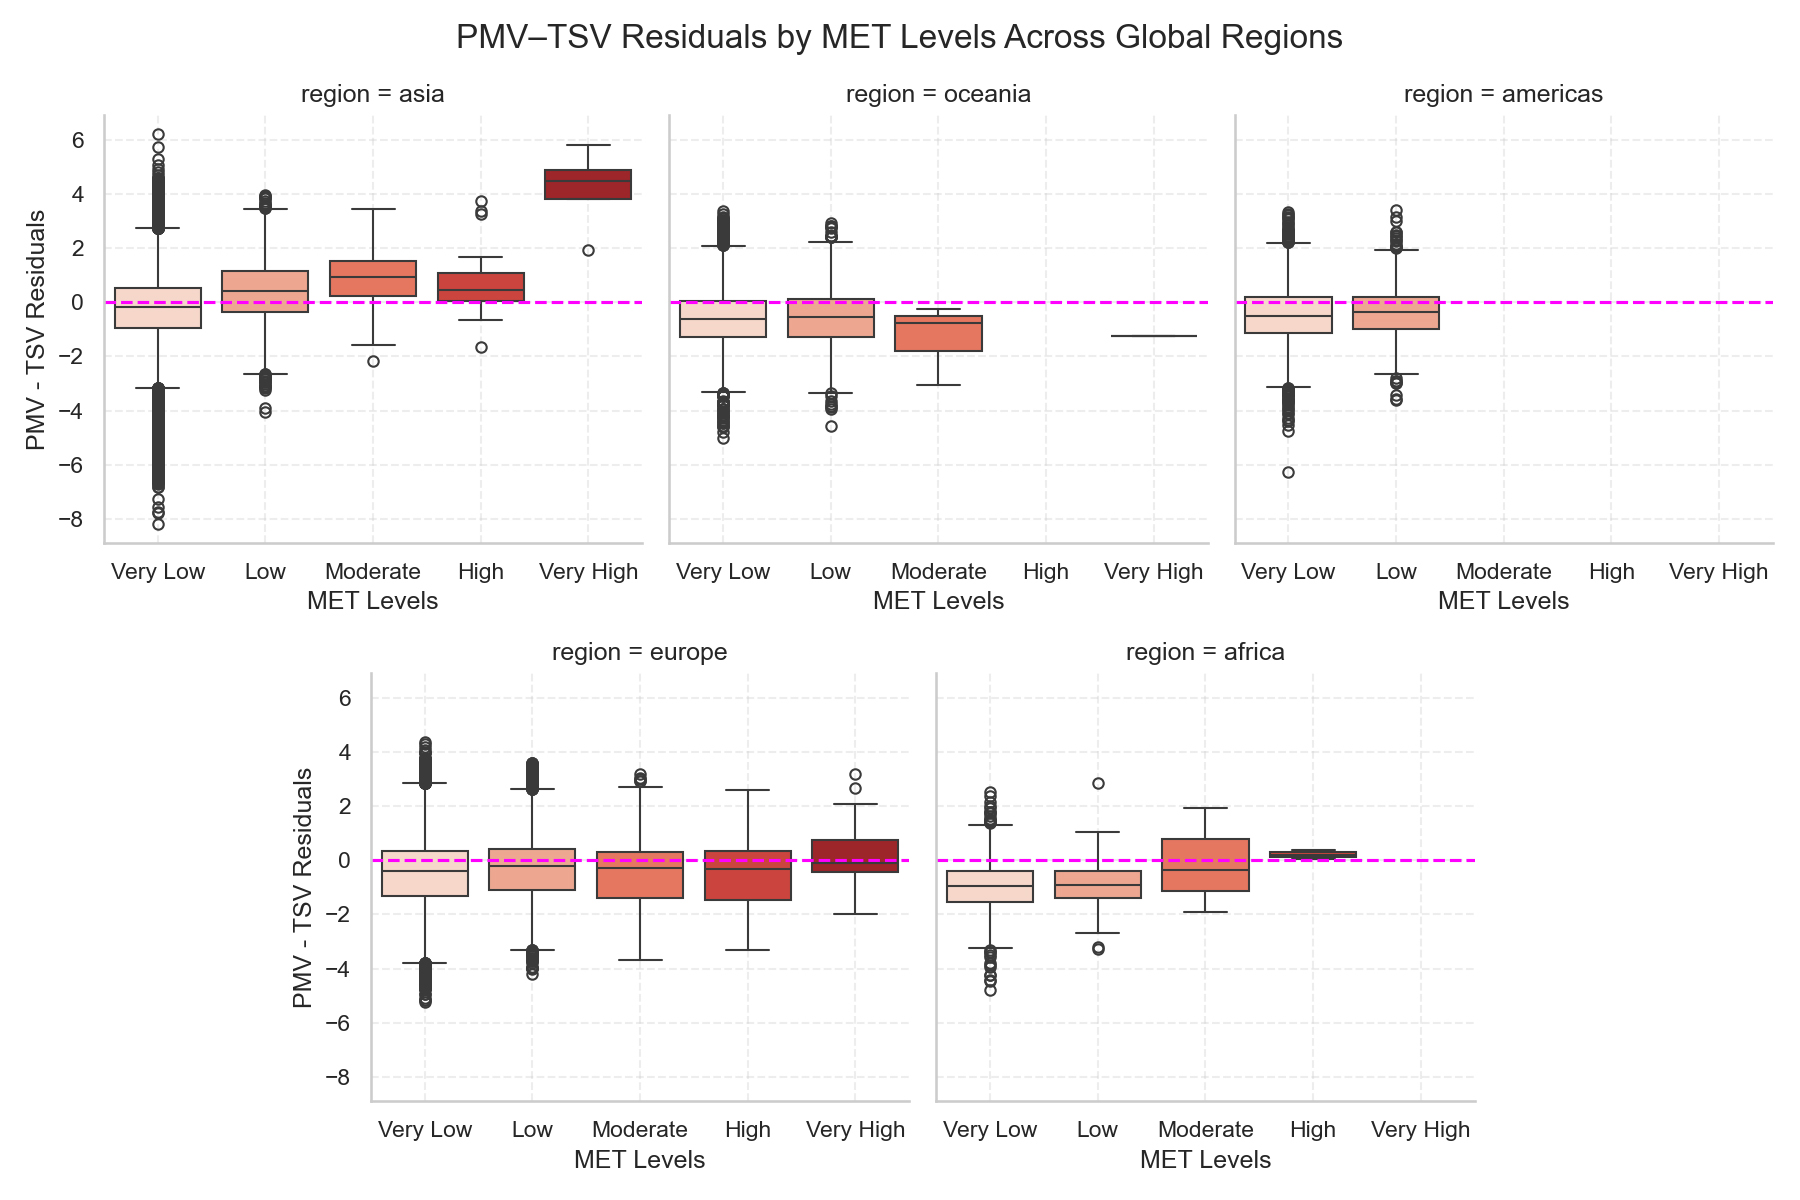
\includegraphics[width=1.0\linewidth]{facet_met_residuals_new.jpg}
    \caption{Box plot of the differences between PMV and TSV across MET with respect to different regions}
    \label{8}
\end{figure}

Figure~\ref{8} illustrates the differences in TSV and PMV based on MET in different regions. The red dashed line corresponds to a residual of 0, indicating the highest accuracy of PMV at this point. As the residual increases, the accuracy of PMV gradually decreases. Overall, the MET class corresponding to the best alignment between TSV and PMV. For Oceania, the PMV prediction is most accurate when MET is very high. For the Americas, Europe, and Africa, the most accurate PMV prediction occurs when MET is high, while for Asia, it is most accurate when MET is medium. This indicates that the level of MET significantly affects the accuracy of PMV predictions, with PMV predictions being more accurate when MET is higher compared to when it is lower. Particularly, among the five regions, there is not much difference in PMV accuracy when MET is low or medium. When the human metabolic rate is low, PMV generally tends to be lower than TSV, whereas when the metabolic rate is high, PMV tends to be higher than TSV.

\begin{figure}[h!]
    \centering
    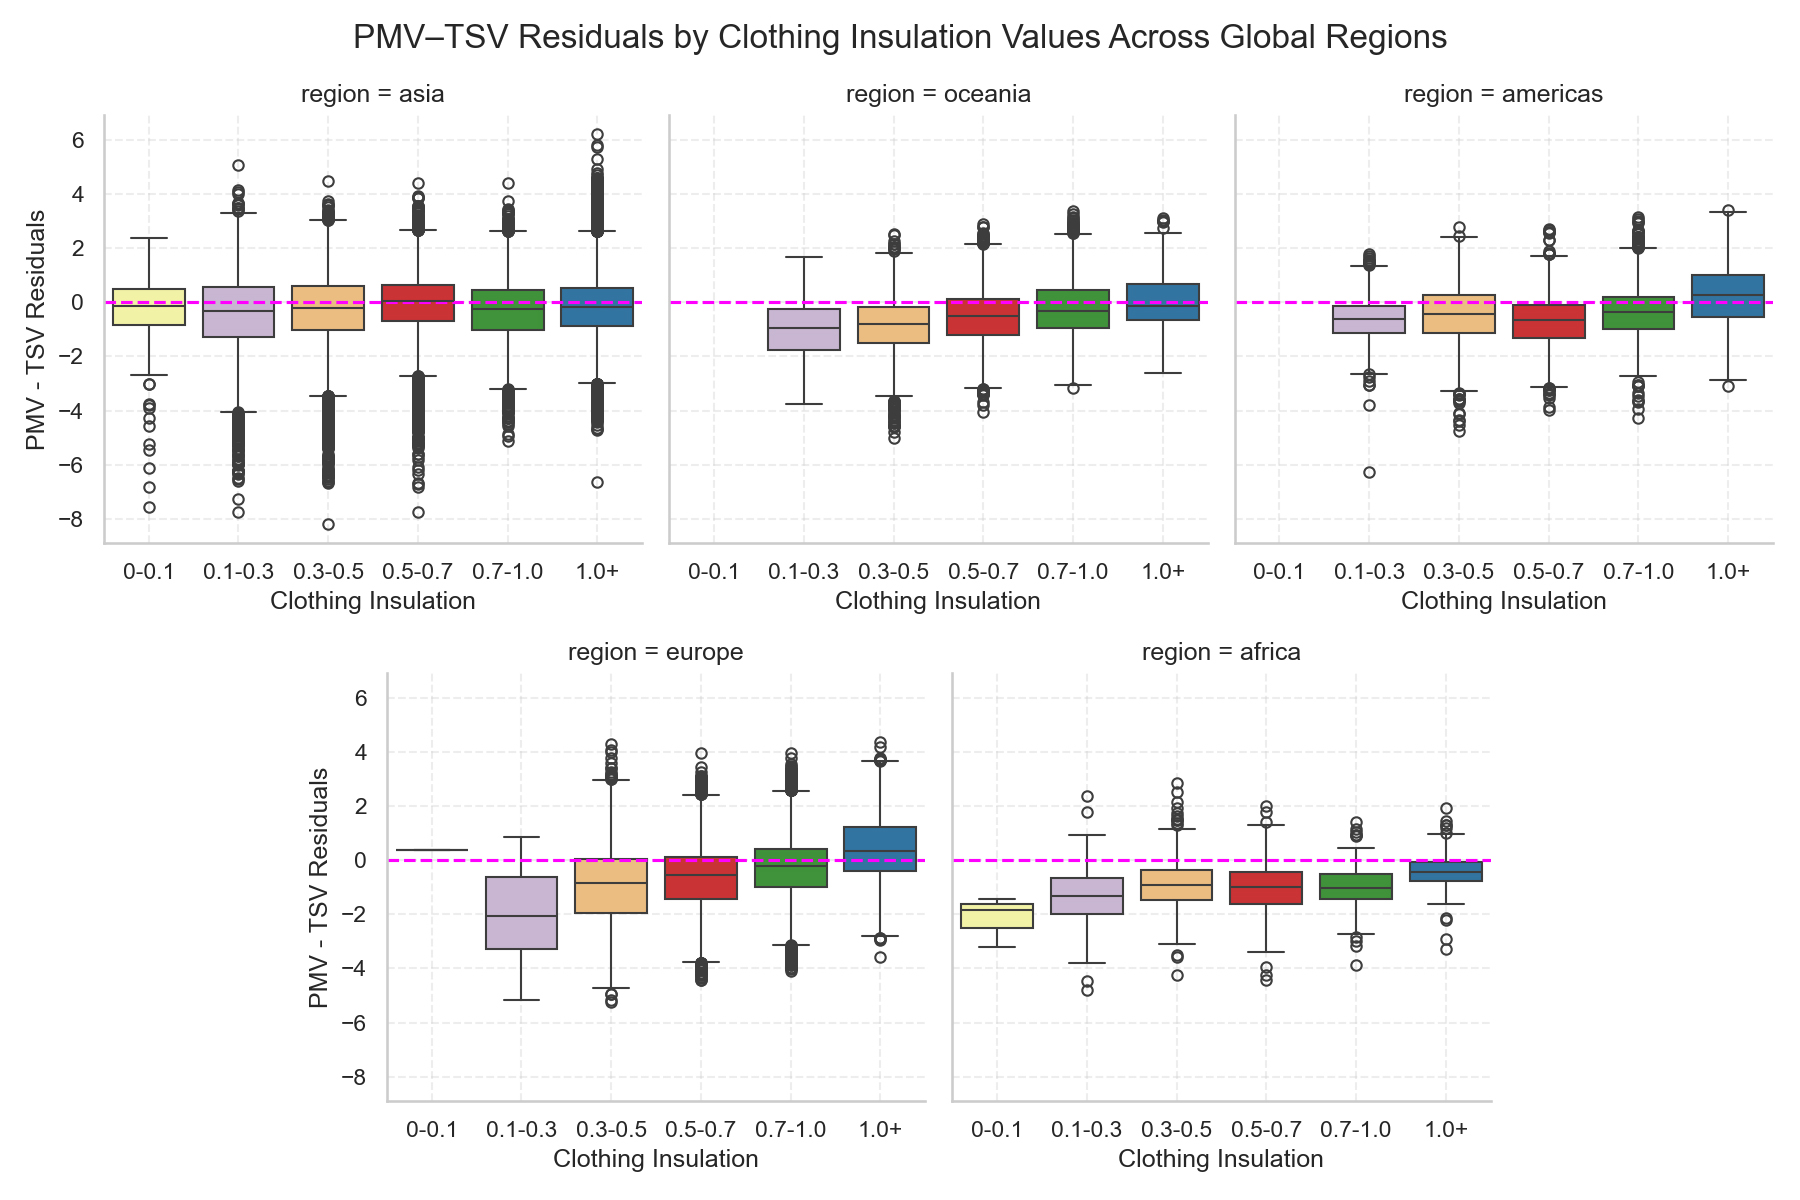
\includegraphics[width=1.0\linewidth]{facet_clo_residuals_new.jpg}
    \caption{Box plot of the differences between PMV and TSV across CLO with respect to different regions}
    \label{9}
\end{figure}

Furthermore, the impact of different MET values on PMV residuals varies across regions. In Oceania, PMV values are generally lower than TSV, indicating that the predicted values are lower than the actual thermal sensation of individuals. They are only equal to TSV when MET is very high, with residuals not exceeding -1, and minimal differences between low and high MET levels. In the Americas, with no instances of very high MET, the impact of MET on TSV residuals is relatively uniform, with differences of about 0.5 between adjacent MET intervals. For Europe, residuals gradually decrease with increasing MET, reaching a minimum at High levels and then increasing again at very high MET levels. Asia's data is the most scattered, especially at MET very low, where extreme values appear, with residuals ranging from -8 to 6, but the mean remains around -0.5, indicating that PMV predictions are mostly accurate in reflecting thermal sensation votes at this point. In contrast, Africa's data is more concentrated, partly due to the smaller dataset. However, in very high MET situations, PMV residuals can reach up to 2, suggesting that PMV predictions are not suitable for high metabolic activities in Africa. Overall, PMV is more suitable for moderate-intensity activities, with less reliability in predicting values for low and high-intensity activities.

Similarly, the differences in PMV prediction accuracy based on CLO in different regions are shown in Figure~\ref{9}. Due to the lack of data for Europe and Africa, this section only discusses the differences among the Americas, Oceania, and Asia. It is evident that most experiments in the Americas were conducted in summer, leading to a lack of winter CLO data. When CLO is between 0.3-0.5, PMV predictions are accurate, but when CLO is between 0.1-0.3, PMV residuals are larger. In Oceania, PMV values are generally lower than TSV, with residuals decreasing as CLO increases, and the most accurate PMV predictions occur when CLO is greater than 1.0. In Asia, the mean PMV residuals are mostly between -1 and 1, indicating that most PMV predictions are accurate, with the most accurate predictions occurring when CLO is between 0.5-0.7.

Overall, the CLO ranges vary across different regions, with Oceania having the widest range, followed by Asia and the Americas. For the Americas and Oceania, there is a more noticeable pattern between CLO and PMV prediction accuracy, where higher CLO values correspond to more accurate TSV predictions. However, in Asia, while CLO does impact TSV prediction accuracy, the differences are not significant and lack a clear pattern. Therefore, for different regions, the CLO ranges suitable for PMV vary, and the impact of CLO differs as well. This suggests that the standardized clothing thermal resistance may not be applicable to subjects from different regions. Future research should measure different clothing thermal resistances based on the populations in different regions to reduce limitations in thermal sensation predictions.

\subsection{Preliminary Adaptive Comfort Modeling in Chinese Climate Zones}

Following the methodology of de Dear et al.~\cite{dedearDevelopingAdaptiveModel1998}, we conducted a preliminary regression analysis to derive zone-specific adaptive comfort models from the Chinese Thermal Comfort Dataset. We restricted our dataset to naturally ventilated buildings and selected records with thermal sensation votes near neutrality ($|\mathrm{TSV}| \leq 0.5$). For approximately 60\% of these cases, outdoor air temperature was available, enabling linear regressions of indoor neutral temperature against outdoor conditions. For the remaining 40\%, we report descriptive indoor air temperatures corresponding to neutral thermal sensation.

\begin{table}[h!]
\centering
\caption{Zone-specific adaptive thermal comfort regressions ($T_{\text{neutral}} = a \cdot T_{\text{out}} + b$)}
\label{tab:adaptive-regression}
\begin{tabular}{lccc}
\toprule
\textbf{Climate Zone} & \textbf{Slope ($a$)} & \textbf{Intercept ($b$)} & \textbf{$R^2$} \\
\midrule
Cold zone & 0.502 & 14.577 & 0.67 \\
Hot summer and cold winter zone & 0.617 & 12.332 & 0.82 \\
Hot summer and warm winter zone & 0.819 & 6.818 & 0.71 \\
Severe cold zone & 0.196 & 22.078 & 0.53 \\
\bottomrule
\end{tabular}
\end{table}

\begin{table}[h!]
\centering
\caption{Mean indoor air temperature at TSV $\approx$ 0 in fallback (no $T_{\text{out}}$) cases}
\label{tab:neutral-fallback}
\begin{tabular}{lccc}
\toprule
\textbf{Climate Zone} & \textbf{Mean ($^\circ$C)} & \textbf{Std Dev} & \textbf{Sample Size} \\
\midrule
Cold zone & 21.43 & 4.56 & 413 \\
Hot summer and cold winter zone & 22.17 & 5.42 & 3264 \\
Hot summer and warm winter zone & 21.96 & 2.86 & 10 \\
Mild zone & 20.67 & 4.64 & 415 \\
Severe cold zone & 21.88 & 1.97 & 139 \\
\bottomrule
\end{tabular}
\end{table}


As shown in Table~\ref{tab:adaptive-regression}, fitted slopes vary across zones, with the ``hot summer and warm winter'' zone exhibiting the highest adaptation slope ($0.819$), suggesting stronger behavioral adaptation to outdoor temperature. In contrast, the ``severe cold zone'' shows a much flatter response ($0.196$), likely reflecting more tightly controlled indoor environments or reduced adaptive behaviors. Descriptive statistics for fallback cases (Table~\ref{tab:neutral-fallback}) also show zone-specific variation in indoor neutral temperatures, with ``mild zone'' records averaging around $20.7\,^\circ$C. These findings underscore the importance of regionally adaptive thermal comfort models within China.

\subsection{Subjectivity of Evaluation Metrics}

While our study adopts a structured qualitative scoring method rather than quantitative modeling or meta-analysis, this approach was purposefully designed to expose systemic blind spots across the literature in a reproducible manner. Unlike Sun et al.\cite{Sun2019ImprovedPMV}, which focused on refining PMV within naturally ventilated contexts using localized factors, our review spans 88 studies across two major thermal comfort databases and includes 15 variables grouped into personal, contextual, and PMV-specific categories. This comparative breadth allows us to surface discrepancies in parameter usage, reporting standards, and regional modeling assumptions that have been underexplored in previous literature. We acknowledge that numerical evaluation inherently involves a degree of subjectivity; however, we mitigated this through well-defined rating criteria and cross-sectional consistency checks. Future studies may expand upon this work by introducing inter-rater reliability assessments or applying statistical tests to evaluate the impact of parameter inclusion on prediction error. Nonetheless, the strength of our method lies in its ability to unify and evaluate highly heterogeneous studies within a coherent, comparable framework—something existing modeling studies often overlook.

\section{Conclusion}
\label{sec1}

This review paper is an attempt to analyze and compare the thermal comfort studies covered in the ASHRAE Global Thermal Comfort Database and the Chinese Thermal Comfort Dataset from a data-driven qualitative perspective. Our analysis reveals that current research utilizing these two thermal comfort databases primarily focuses on four key areas: 
(1) fundamental questions to the nature of the two databases, 
(2) looking for improved thermal comfort modeling techniques upon PMV values, 
(3) data mining on thermal comfort database records, and
(4) improvement of international design standards.
However, our review process uncovered significant challenges in comparing thermal comfort studies across the two databases due to inconsistencies in methodologies and reporting.
The deficiency of a universally standardized classification system applicable across all global regions poses challenges in the assessment and amalgamation of thermal comfort data. Furthermore, we found that current studies based on the two thermal comfort databases place less emphasis on regional, cultural, and individual characteristics. 
To address these issues, we conducted an in-depth review of 88 articles from three sources (ASHRAE, Chinese, and additional databases), examining how they incorporate personal characteristics, contextual parameters, and PMV calculation inputs in thermal comfort analyses.


Regarding personal characteristics, the five parameters - age, gender, height, weight, and Body Mass Index (BMI) - pertaining to personal characteristics outlined in Section B are not fully considered in the analysis of thermal comfort. 
Criteria for categorizing age groups, for example, varied significantly across studies, likely due to the wide range of ages represented across studies thereby across the datasets.
Lack of universally accepted standard for age groupings in thermal comfort surveys worldwide makes it challenging to conduct comparative studies across different databases.
The results also indicate that the age range of the subjects in the reviewed studies was primarily concentrated between 18-25 years old, lacking the composition of data from older adults and children. 
Furthermore, these findings suggest that gender could be a critical factor in predicting thermally driven behaviors and should be considered by thermal comfort models.
Moving onward to the outcomes related to height, weight, and BMI, all three parameters are insufficiently examined in thermal comfort research, with BMI receiving even less attention.

Compared to personal characteristics, contextual parameters have gained more focus through previous research. The review results indicate that approximately half of the reviewed articles examined variations in contextual parameters concerning thermal comfort. Nevertheless, the primary challenges identified revolve around mapping discrepancies within the three contextual parameters of climate zone, building type, and operation mode. Due to variations in categorization methods for these parameters across the two databases, the integration and analysis of thermal comfort data from global regions were hindered, limiting the ability to systematically compare and evaluate them. We suggest an enhancement and augmentation to the existing version of the ASHRAE Standard 55 by introducing a standardized classification system for contextual parameters that is applicable across all global regions.

In terms of inputs for the PMV calculation, these six parameters received the most attention across all the examined articles. Although the research on the impact of air temperature, air velocity, and relative humidity on thermal comfort is relatively comprehensive and substantial, MRT is not as emphasized as other parameters, which is also evident in the review results. We suggest future research should pay more attention to the impact of MRT. This focus can provide guidance for designing pleasurable indoor environments based on a more thorough understanding of MRT's influence. Additionally, we observed that researchers tend to use a uniform value to represent the results when considering the impact of metabolism, which is not accurate and appropriate.

Our study also evaluates beyond prior investigations, offering a broader set of modeling variables across two thermal comfort databases and five Chinese climate zones, revealing systemic gaps in demographic and contextual representation. By systematically scoring studies on 15 distinct parameters—including PMV inputs, personal demographics, and contextual attributes—we reveal structural limitations in current datasets and modeling practices. In particular, our comparative modeling of Chinese climate zones demonstrates how region-specific adaptations can shift thermal expectations. These insights directly support the design of more flexible, occupant-responsive HVAC control strategies—an essential step in aligning thermal comfort research with the operational dynamics of renewable energy systems. A standardized, culturally adaptive comfort framework is thus critical not only for advancing building design, but for accelerating the decarbonization of indoor environmental systems.


\appendix
\section{Full Data Not-Null Availability Heatmap}
To complement Figure~\ref{1} where we only showed a handful of columns inside the combined dataset, we are showing the full data availability heatmap here with Figure~\ref{fig:fullavail}. To provide a better context of what kind of climate zones are included across the combined dataset, we have also created, along similar notes the number of records within each climate zone within the combined dataset in Figure~\ref{fig:czrecords}.
\begin{figure}[h!]
    \centering
    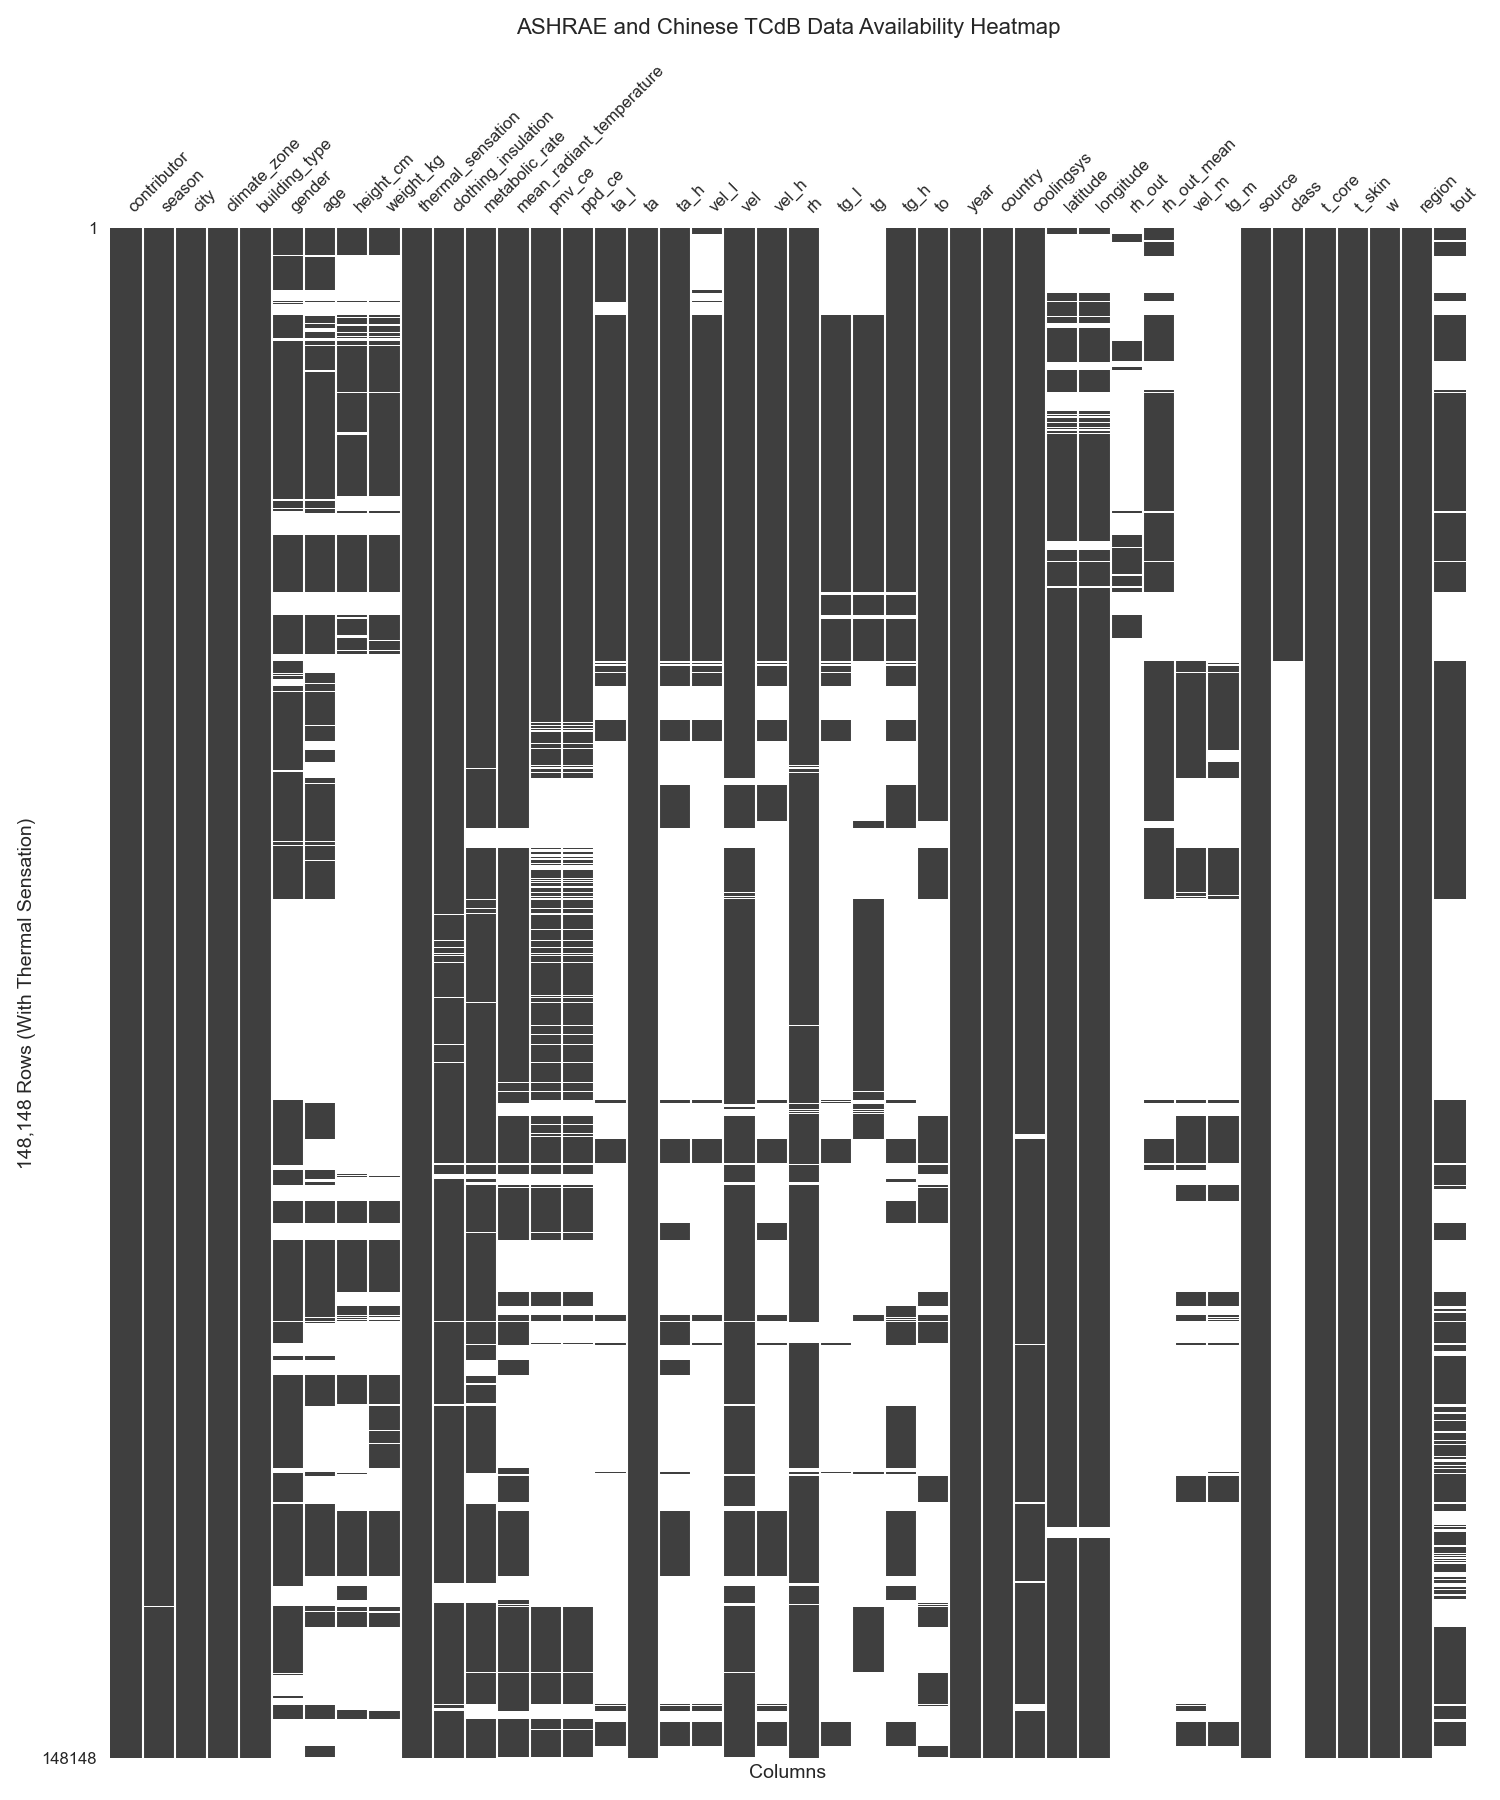
\includegraphics[width=0.85\linewidth]{FullFill.png}
    \caption{Complete heatmap of all columns of the combined dataset}
    \label{fig:fullavail}
\end{figure}

\begin{figure}
    \centering
    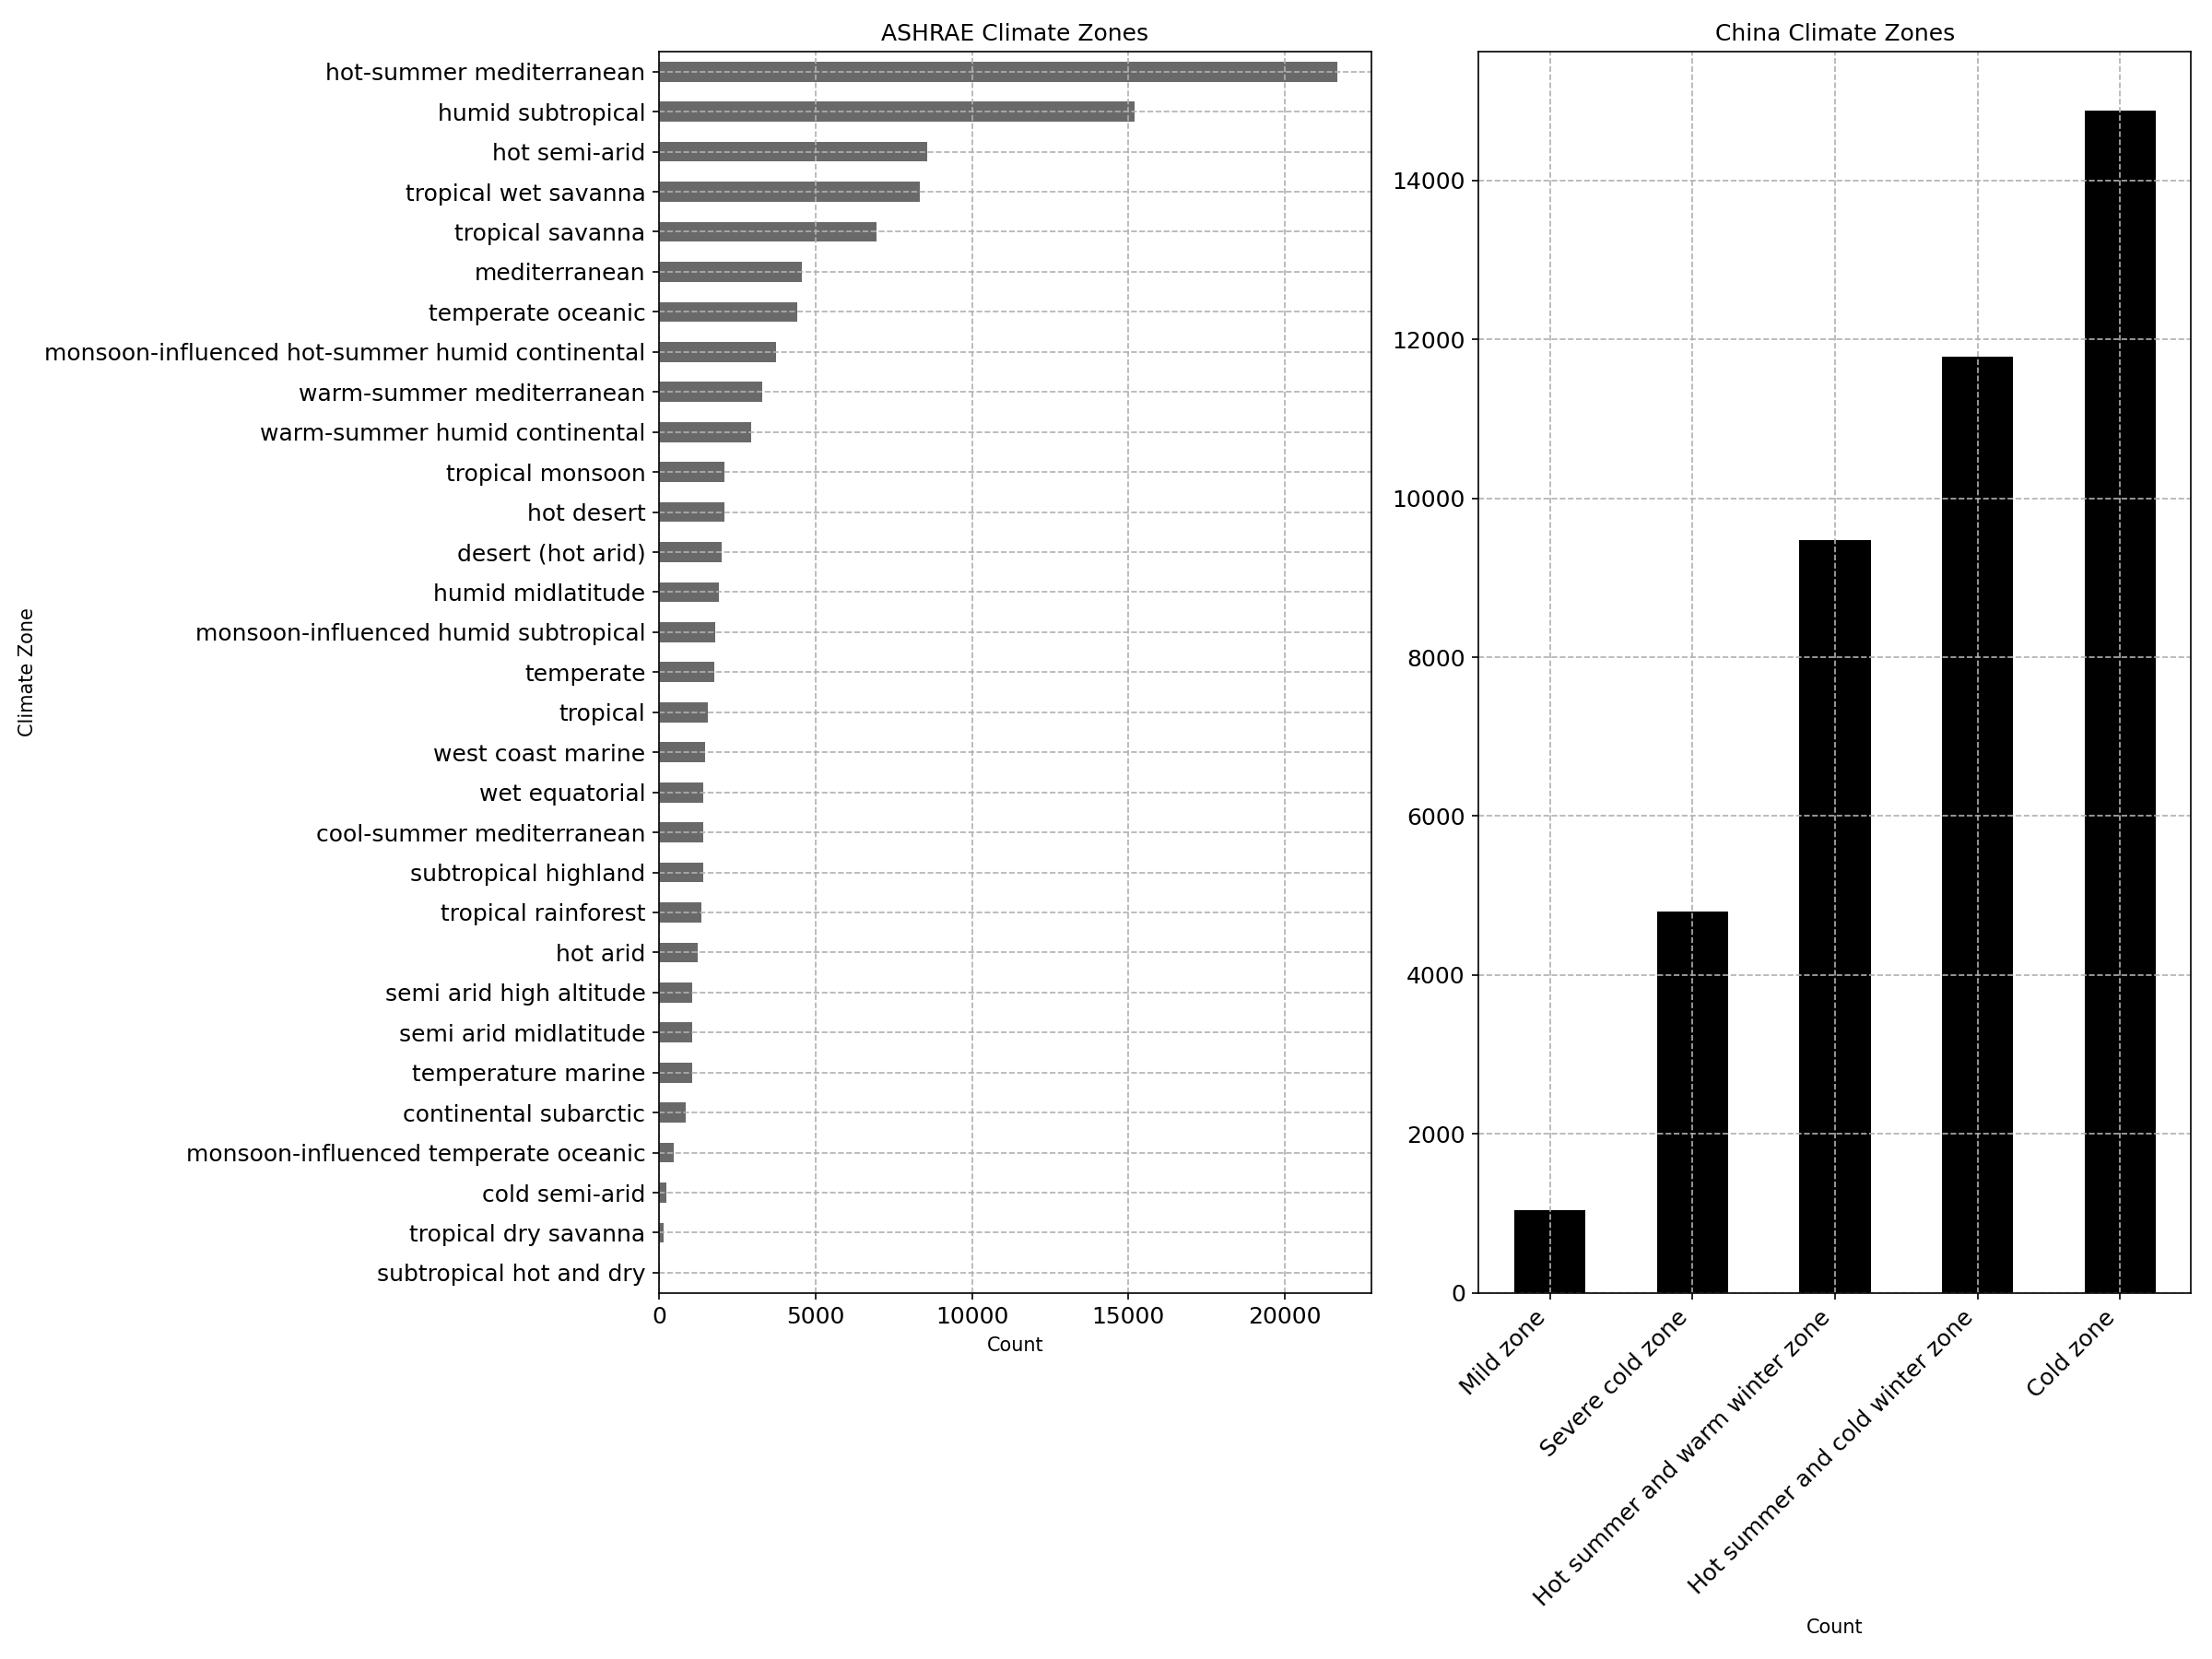
\includegraphics[width=1.0\linewidth]{climate_records.png}
    \caption{Number of records within climate zone in the ASHRAE and Chinese thermal comfort databases respectively}
    \label{fig:czrecords}
\end{figure}

\clearpage
\section{Complete Correlation Matrix for Selected Parameters}
\begin{figure}[h!]
    \centering
    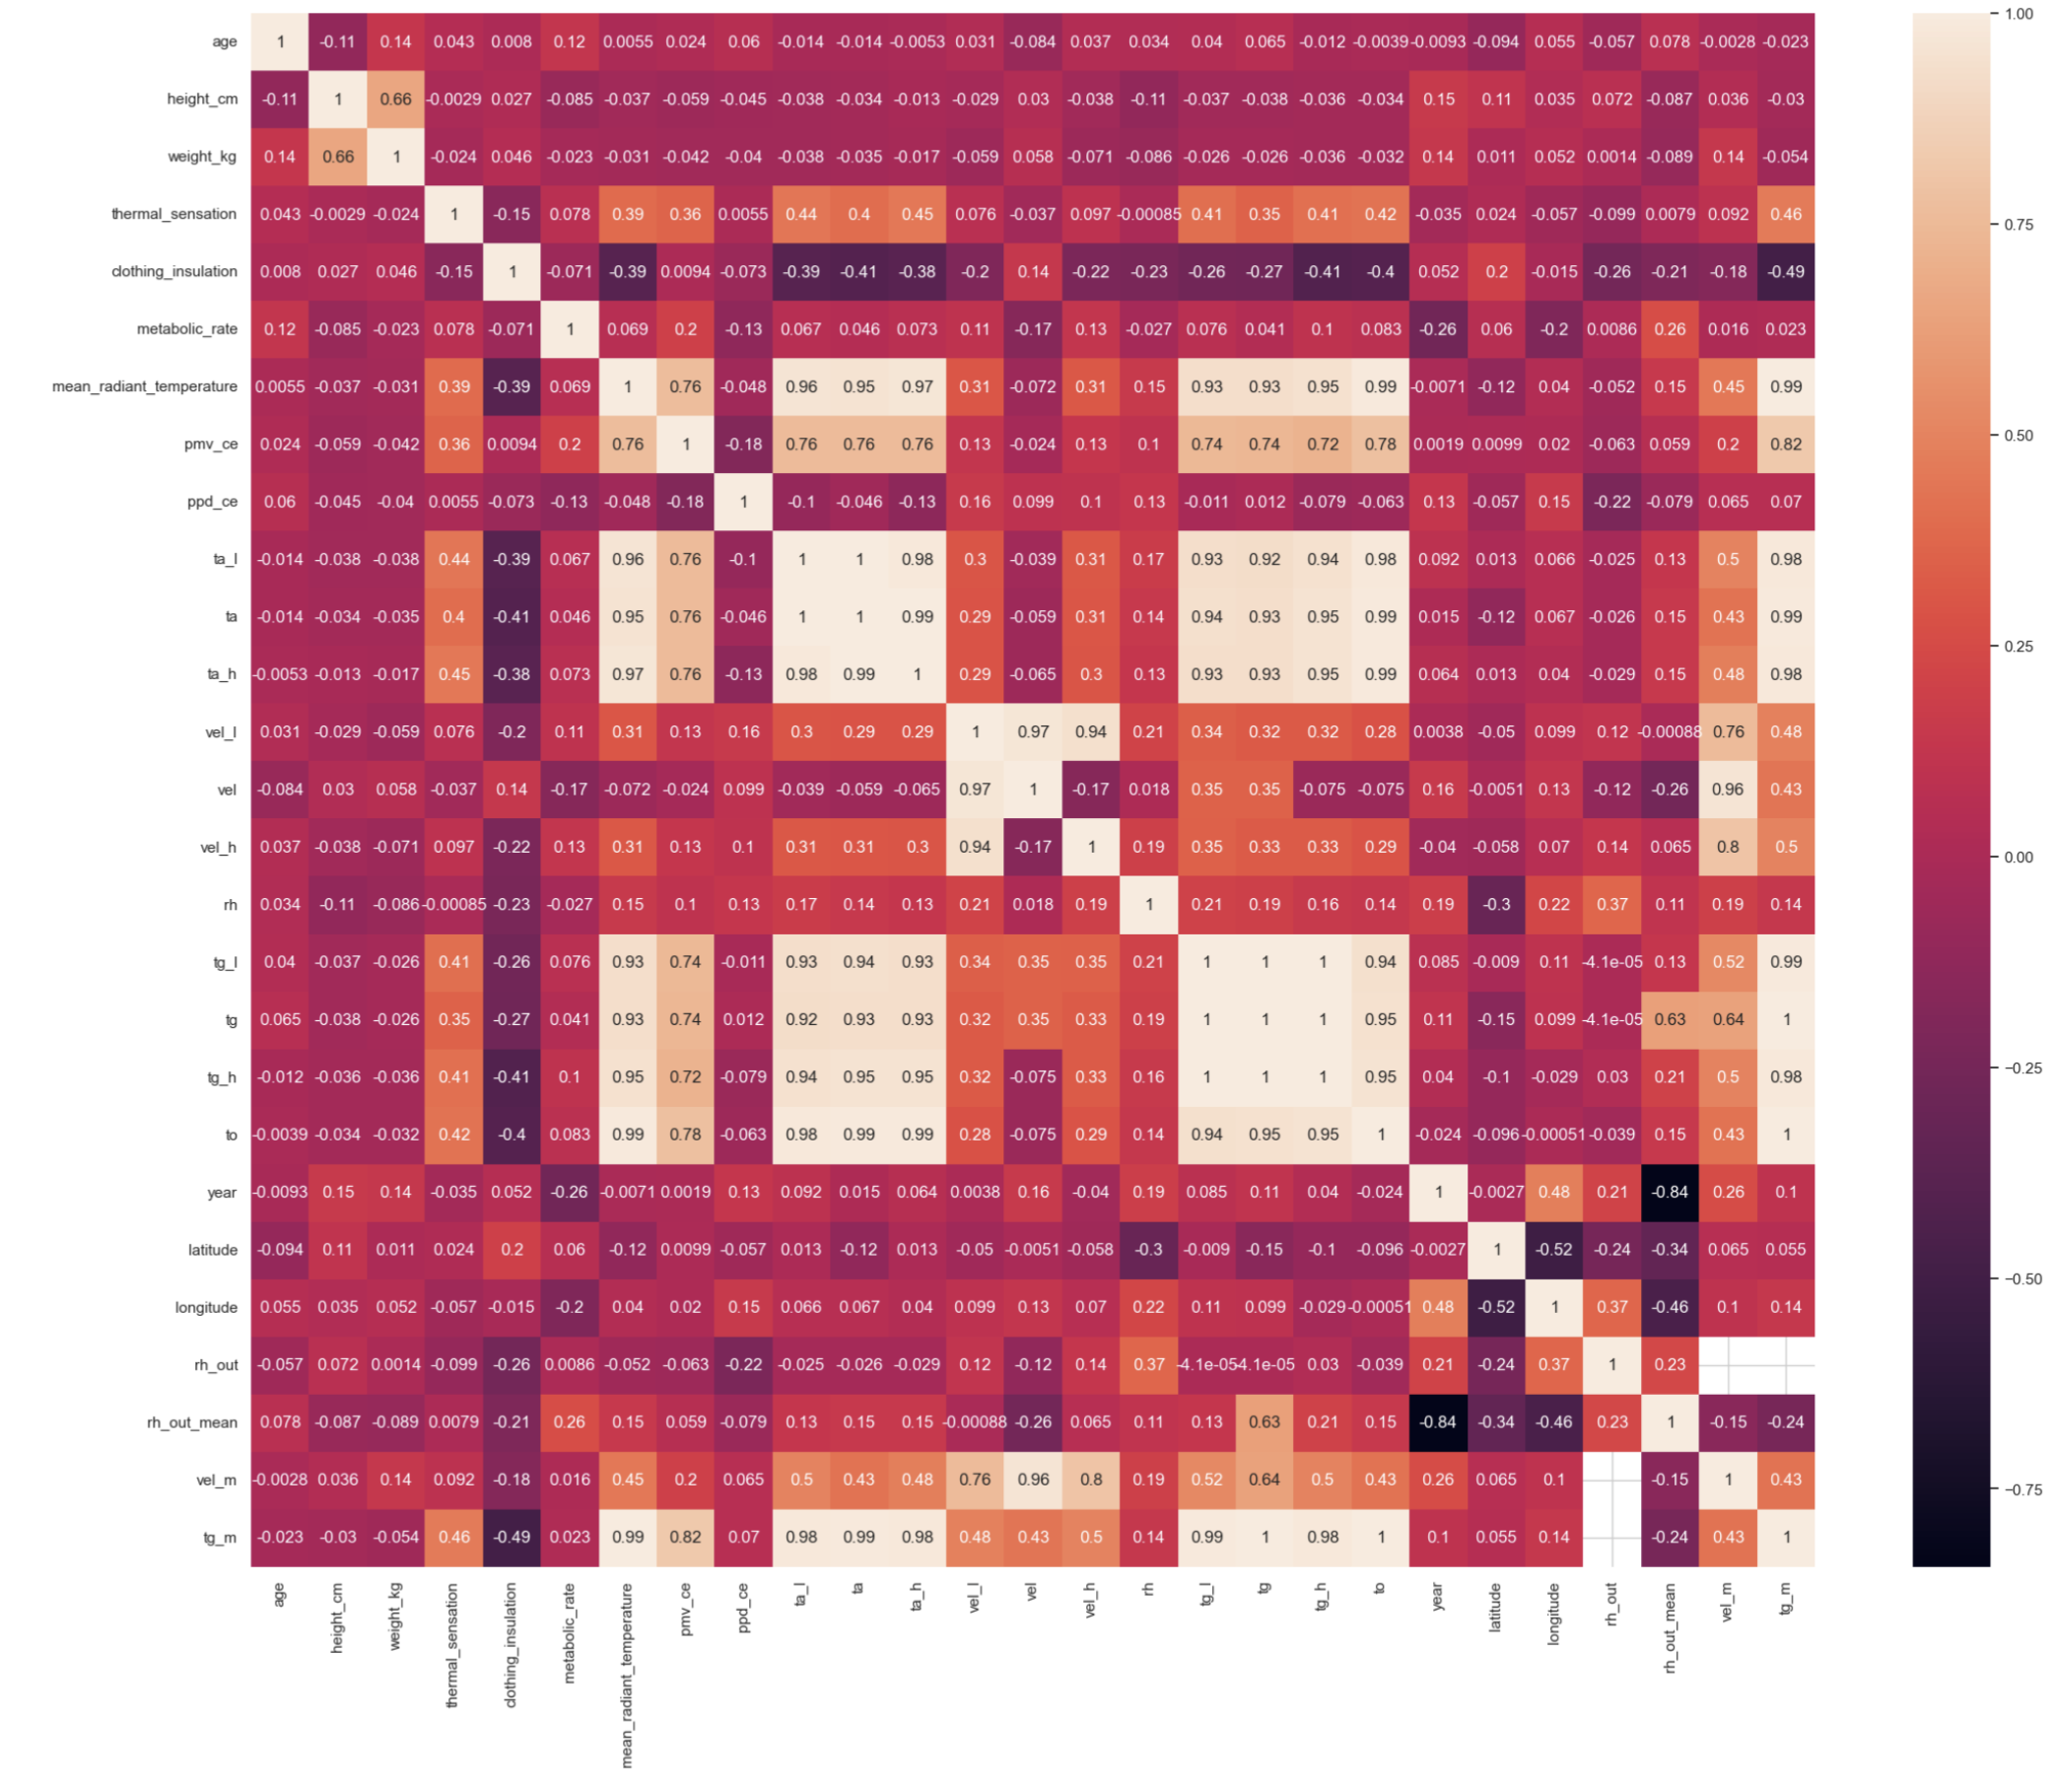
\includegraphics[width=1.0\linewidth]{correlation matrix.png}
    \caption{Correlation matrix for selected parameters}
    \label{correlation}
\end{figure}

\bibliographystyle{elsarticle-num} 
\clearpage
\bibliography{cas-refs}

\end{document}

\endinput
%%
%% End of file `elsarticle-template-num.tex'.
